\documentclass[twoside]{book}

% Packages required by doxygen
\usepackage{calc}
\usepackage{doxygen}
\usepackage{graphicx}
\usepackage[utf8]{inputenc}
\usepackage{makeidx}
\usepackage{multicol}
\usepackage{multirow}
\usepackage{textcomp}
\usepackage[table]{xcolor}

% NLS support packages
\usepackage[french]{babel}

% Font selection
\usepackage[T1]{fontenc}
\usepackage{mathptmx}
\usepackage[scaled=.90]{helvet}
\usepackage{courier}
\usepackage{amssymb}
\usepackage{sectsty}
\renewcommand{\familydefault}{\sfdefault}
\allsectionsfont{%
  \fontseries{bc}\selectfont%
  \color{darkgray}%
}
\renewcommand{\DoxyLabelFont}{%
  \fontseries{bc}\selectfont%
  \color{darkgray}%
}

% Page & text layout
\usepackage{geometry}
\geometry{%
  a4paper,%
  top=2.5cm,%
  bottom=2.5cm,%
  left=2.5cm,%
  right=2.5cm%
}
\tolerance=750
\hfuzz=15pt
\hbadness=750
\setlength{\emergencystretch}{15pt}
\setlength{\parindent}{0cm}
\setlength{\parskip}{0.2cm}
\makeatletter
\renewcommand{\paragraph}{%
  \@startsection{paragraph}{4}{0ex}{-1.0ex}{1.0ex}{%
    \normalfont\normalsize\bfseries\SS@parafont%
  }%
}
\renewcommand{\subparagraph}{%
  \@startsection{subparagraph}{5}{0ex}{-1.0ex}{1.0ex}{%
    \normalfont\normalsize\bfseries\SS@subparafont%
  }%
}
\makeatother

% Headers & footers
\usepackage{fancyhdr}
\pagestyle{fancyplain}
\fancyhead[LE]{\fancyplain{}{\bfseries\thepage}}
\fancyhead[CE]{\fancyplain{}{}}
\fancyhead[RE]{\fancyplain{}{\bfseries\leftmark}}
\fancyhead[LO]{\fancyplain{}{\bfseries\rightmark}}
\fancyhead[CO]{\fancyplain{}{}}
\fancyhead[RO]{\fancyplain{}{\bfseries\thepage}}
\fancyfoot[LE]{\fancyplain{}{}}
\fancyfoot[CE]{\fancyplain{}{}}
\fancyfoot[RE]{\fancyplain{}{\bfseries\scriptsize Généré le Dimanche 20 Mars 2016 18\-:34\-:56 pour Solf\-Help par Doxygen }}
\fancyfoot[LO]{\fancyplain{}{\bfseries\scriptsize Généré le Dimanche 20 Mars 2016 18\-:34\-:56 pour Solf\-Help par Doxygen }}
\fancyfoot[CO]{\fancyplain{}{}}
\fancyfoot[RO]{\fancyplain{}{}}
\renewcommand{\footrulewidth}{0.4pt}
\renewcommand{\chaptermark}[1]{%
  \markboth{#1}{}%
}
\renewcommand{\sectionmark}[1]{%
  \markright{\thesection\ #1}%
}

% Indices & bibliography
\usepackage{natbib}
\usepackage[titles]{tocloft}
\setcounter{tocdepth}{3}
\setcounter{secnumdepth}{5}
\makeindex

% Custom commands
\newcommand{\clearemptydoublepage}{%
  \newpage{\pagestyle{empty}\cleardoublepage}%
}


%===== C O N T E N T S =====

\begin{document}

% Titlepage & ToC
\pagenumbering{roman}
\begin{titlepage}
\vspace*{7cm}
\begin{center}%
{\Large Solf\-Help }\\
\vspace*{1cm}
{\large Généré par Doxygen 1.8.6}\\
\vspace*{0.5cm}
{\small Dimanche 20 Mars 2016 18:34:56}\\
\end{center}
\end{titlepage}
\clearemptydoublepage
\tableofcontents
\clearemptydoublepage
\pagenumbering{arabic}

%--- Begin generated contents ---
\chapter{Index hiérarchique}
\section{Hiérarchie des classes}
Cette liste d'héritage est classée approximativement par ordre alphabétique \-:\begin{DoxyCompactList}
\item \contentsline{section}{Note}{\pageref{class_note}}{}
\item Q\-Widget\begin{DoxyCompactList}
\item \contentsline{section}{Accueil}{\pageref{class_accueil}}{}
\item \contentsline{section}{Clavier\-Piano}{\pageref{class_clavier_piano}}{}
\item \contentsline{section}{Cours}{\pageref{class_cours}}{}
\item \contentsline{section}{Entrainement\-Facile}{\pageref{class_entrainement_facile}}{}
\item \contentsline{section}{Entrainement\-Page1}{\pageref{class_entrainement_page1}}{}
\item \contentsline{section}{Fenetre}{\pageref{class_fenetre}}{}
\item \contentsline{section}{Jeu\-Libre}{\pageref{class_jeu_libre}}{}
\end{DoxyCompactList}
\end{DoxyCompactList}

\chapter{Index des classes}
\section{Class List}
Here are the classes, structs, unions and interfaces with brief descriptions\-:\begin{DoxyCompactList}
\item\contentsline{section}{{\bf Accueil} }{\pageref{class_accueil}}{}
\item\contentsline{section}{{\bf Clavier\-Piano} }{\pageref{class_clavier_piano}}{}
\item\contentsline{section}{{\bf Cours} }{\pageref{class_cours}}{}
\item\contentsline{section}{{\bf Entrainement\-Facile} }{\pageref{class_entrainement_facile}}{}
\item\contentsline{section}{{\bf Entrainement\-Page1} }{\pageref{class_entrainement_page1}}{}
\item\contentsline{section}{{\bf Fenetre} }{\pageref{class_fenetre}}{}
\item\contentsline{section}{{\bf Jeu\-Libre} }{\pageref{class_jeu_libre}}{}
\item\contentsline{section}{{\bf Note} }{\pageref{class_note}}{}
\end{DoxyCompactList}

\chapter{Documentation des classes}
\section{Référence de la classe Accueil}
\label{class_accueil}\index{Accueil@{Accueil}}
Graphe d'héritage de Accueil\-:\begin{figure}[H]
\begin{center}
\leavevmode
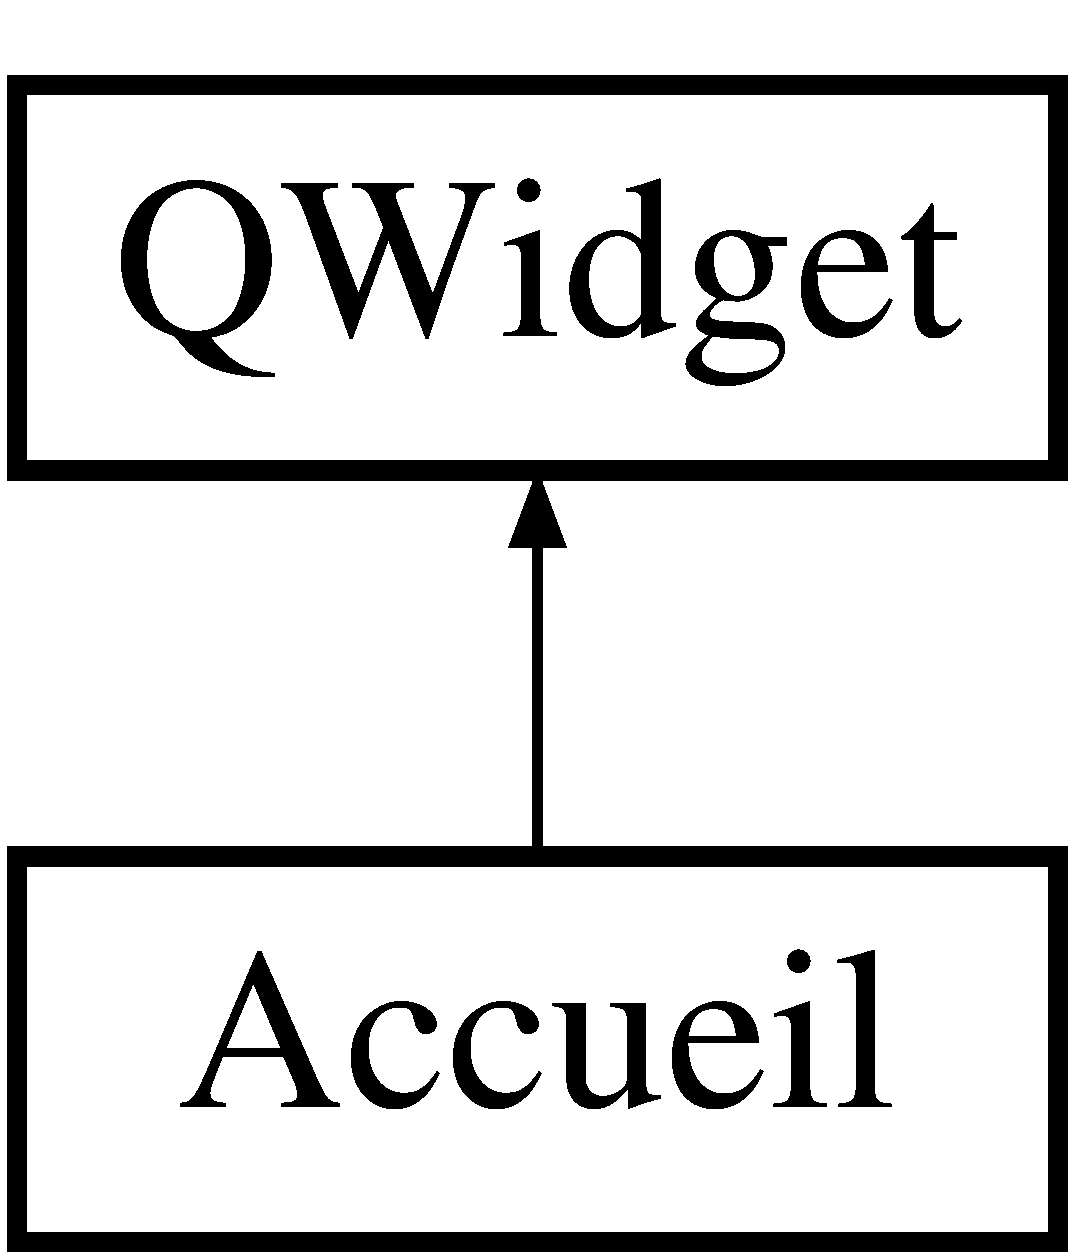
\includegraphics[height=2.000000cm]{class_accueil}
\end{center}
\end{figure}
\subsection*{Connecteurs publics}
\begin{DoxyCompactItemize}
\item 
void {\bf do\-Cours} ()
\begin{DoxyCompactList}\small\item\em Fonction qui permet d'accéder à la fenetre de cours. \end{DoxyCompactList}\item 
void {\bf do\-Entrainement} ()
\begin{DoxyCompactList}\small\item\em Fonction qui permet d'accéder à la fen$^\wedge$etre d'entrainement. \end{DoxyCompactList}\item 
void {\bf do\-Libre} ()
\begin{DoxyCompactList}\small\item\em Fonction qui permet d'accéder à la fenetre de jeu libre. \end{DoxyCompactList}\end{DoxyCompactItemize}
\subsection*{Fonctions membres publiques}
\begin{DoxyCompactItemize}
\item 
{\bf Accueil} (Q\-Stacked\-Widget $\ast$p)
\begin{DoxyCompactList}\small\item\em Constructeur. \end{DoxyCompactList}\item 
void {\bf ecrire\-Log} (Q\-String s)
\begin{DoxyCompactList}\small\item\em Fonction qui ouvre le fichier de log afin d'y ajouter la chaine de caractère passée en paramètre. \end{DoxyCompactList}\end{DoxyCompactItemize}


\subsection{Documentation des constructeurs et destructeur}
\index{Accueil@{Accueil}!Accueil@{Accueil}}
\index{Accueil@{Accueil}!Accueil@{Accueil}}
\subsubsection[{Accueil}]{\setlength{\rightskip}{0pt plus 5cm}void Accueil\-::\-Accueil (
\begin{DoxyParamCaption}
\item[{Q\-Stacked\-Widget $\ast$}]{p}
\end{DoxyParamCaption}
)}\label{class_accueil_a00bae1419b5ee653b7e0fd6d3abc4449}


Constructeur. 


\begin{DoxyParams}{Paramètres}
{\em p} & Pointeur sur la structure de donnée contenant l'ensemble des fenetre, ne peut etre N\-U\-L\-L \\
\hline
\end{DoxyParams}


\subsection{Documentation des fonctions membres}
\index{Accueil@{Accueil}!do\-Cours@{do\-Cours}}
\index{do\-Cours@{do\-Cours}!Accueil@{Accueil}}
\subsubsection[{do\-Cours}]{\setlength{\rightskip}{0pt plus 5cm}void Accueil\-::do\-Cours (
\begin{DoxyParamCaption}
{}
\end{DoxyParamCaption}
)\hspace{0.3cm}{\ttfamily [slot]}}\label{class_accueil_ada2104f9d052ab3d482d94b530cd574c}


Fonction qui permet d'accéder à la fenetre de cours. 

\begin{DoxyReturn}{Renvoie}
void 
\end{DoxyReturn}
\index{Accueil@{Accueil}!do\-Entrainement@{do\-Entrainement}}
\index{do\-Entrainement@{do\-Entrainement}!Accueil@{Accueil}}
\subsubsection[{do\-Entrainement}]{\setlength{\rightskip}{0pt plus 5cm}void Accueil\-::do\-Entrainement (
\begin{DoxyParamCaption}
{}
\end{DoxyParamCaption}
)\hspace{0.3cm}{\ttfamily [slot]}}\label{class_accueil_a6396dd1af38125e168de6ac7a580a810}


Fonction qui permet d'accéder à la fen$^\wedge$etre d'entrainement. 

\begin{DoxyReturn}{Renvoie}
void 
\end{DoxyReturn}
\index{Accueil@{Accueil}!do\-Libre@{do\-Libre}}
\index{do\-Libre@{do\-Libre}!Accueil@{Accueil}}
\subsubsection[{do\-Libre}]{\setlength{\rightskip}{0pt plus 5cm}void Accueil\-::do\-Libre (
\begin{DoxyParamCaption}
{}
\end{DoxyParamCaption}
)\hspace{0.3cm}{\ttfamily [slot]}}\label{class_accueil_ac7a6e822adc8b61c33382392823bc1e7}


Fonction qui permet d'accéder à la fenetre de jeu libre. 

\begin{DoxyReturn}{Renvoie}
void 
\end{DoxyReturn}
\index{Accueil@{Accueil}!ecrire\-Log@{ecrire\-Log}}
\index{ecrire\-Log@{ecrire\-Log}!Accueil@{Accueil}}
\subsubsection[{ecrire\-Log}]{\setlength{\rightskip}{0pt plus 5cm}void Accueil\-::ecrire\-Log (
\begin{DoxyParamCaption}
\item[{Q\-String}]{s}
\end{DoxyParamCaption}
)}\label{class_accueil_a4090fb7d2fd1ea073f7c6b5488259ee4}


Fonction qui ouvre le fichier de log afin d'y ajouter la chaine de caractère passée en paramètre. 


\begin{DoxyParams}{Paramètres}
{\em s} & une chaine de type Q\-String qui sera écrite dans le fichier log, ne peut etre N\-U\-L\-L \\
\hline
\end{DoxyParams}
\begin{DoxyReturn}{Renvoie}
void 
\end{DoxyReturn}


La documentation de cette classe a été générée à partir des fichiers suivants \-:\begin{DoxyCompactItemize}
\item 
accueil.\-h\item 
accueil.\-cpp\end{DoxyCompactItemize}

\section{Référence de la classe Clavier\-Piano}
\label{class_clavier_piano}\index{Clavier\-Piano@{Clavier\-Piano}}
Graphe d'héritage de Clavier\-Piano\-:\begin{figure}[H]
\begin{center}
\leavevmode
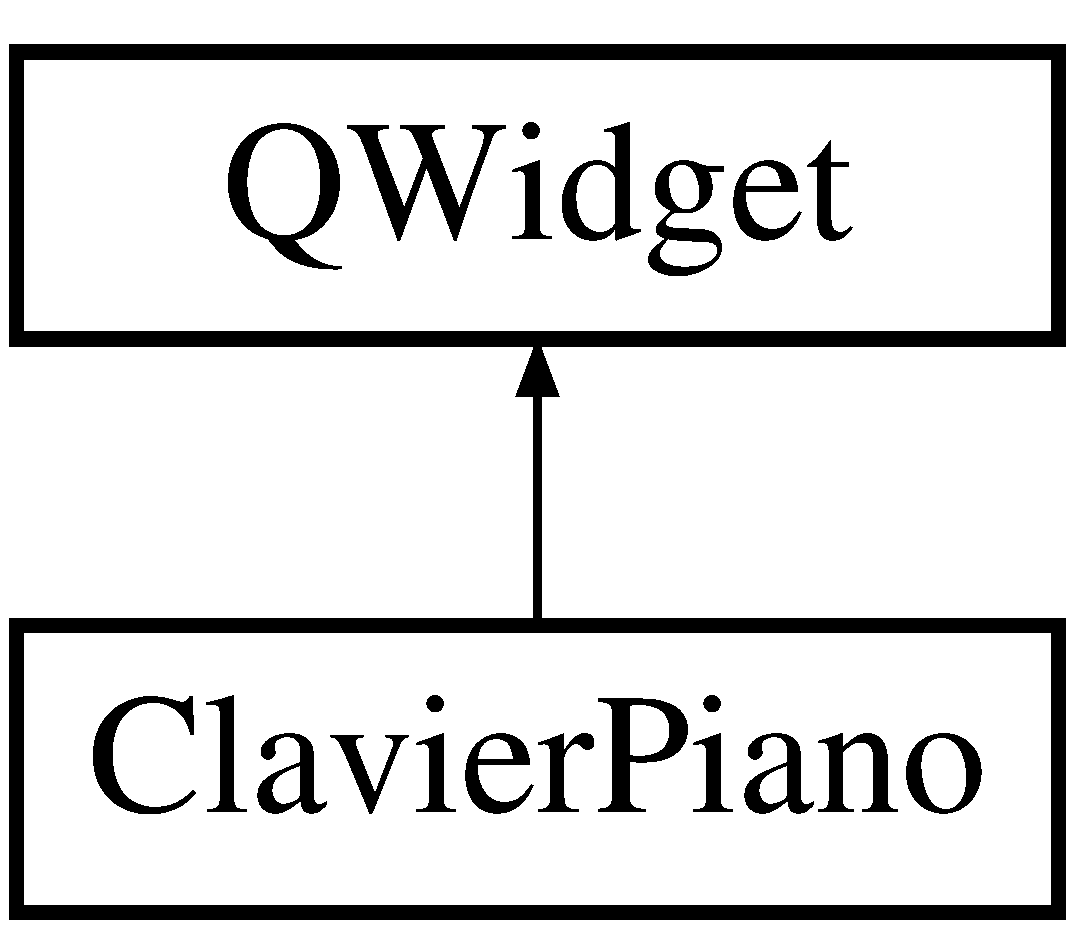
\includegraphics[height=2.000000cm]{class_clavier_piano}
\end{center}
\end{figure}
\subsection*{Connecteurs publics}
\begin{DoxyCompactItemize}
\item 
void {\bf on\-\_\-push\-Button\-Dom\-\_\-clicked} ()
\begin{DoxyCompactList}\small\item\em Fonction qui déclenche le son joué par la touche Do mineur. \end{DoxyCompactList}\item 
void {\bf on\-\_\-push\-Button\-Do\-M\-\_\-clicked} ()
\begin{DoxyCompactList}\small\item\em Fonction qui déclenche le son joué par la touche Do majeur. \end{DoxyCompactList}\item 
void {\bf on\-\_\-push\-Button\-Rem\-\_\-clicked} ()
\begin{DoxyCompactList}\small\item\em Fonction qui déclenche le son joué par la touche Ré mineur. \end{DoxyCompactList}\item 
void {\bf on\-\_\-push\-Button\-Re\-M\-\_\-clicked} ()
\begin{DoxyCompactList}\small\item\em Fonction qui déclenche le son joué par la touche Ré majeur. \end{DoxyCompactList}\item 
void {\bf on\-\_\-push\-Button\-Mim\-\_\-clicked} ()
\begin{DoxyCompactList}\small\item\em Fonction qui déclenche le son joué par la touche mi mineur. \end{DoxyCompactList}\item 
void {\bf on\-\_\-push\-Button\-Mi\-M\-\_\-clicked} ()
\begin{DoxyCompactList}\small\item\em Fonction qui déclenche le son joué par la touche mi majeur. \end{DoxyCompactList}\item 
void {\bf on\-\_\-push\-Button\-Fam\-\_\-clicked} ()
\begin{DoxyCompactList}\small\item\em Fonction qui déclenche le son joué par la touche fa mineur. \end{DoxyCompactList}\item 
void {\bf on\-\_\-push\-Button\-Fa\-M\-\_\-clicked} ()
\begin{DoxyCompactList}\small\item\em Fonction qui déclenche le son joué par la touche fa majeur. \end{DoxyCompactList}\item 
void {\bf on\-\_\-push\-Button\-Solm\-\_\-clicked} ()
\begin{DoxyCompactList}\small\item\em Fonction qui déclenche le son joué par la touche sol mineur. \end{DoxyCompactList}\item 
void {\bf on\-\_\-push\-Button\-Sol\-M\-\_\-clicked} ()
\begin{DoxyCompactList}\small\item\em Fonction qui déclenche le son joué par la touche sol majeur. \end{DoxyCompactList}\item 
void {\bf on\-\_\-push\-Button\-Lam\-\_\-clicked} ()
\begin{DoxyCompactList}\small\item\em Fonction qui déclenche le son joué par la touche la mineur. \end{DoxyCompactList}\item 
void {\bf on\-\_\-push\-Button\-La\-M\-\_\-clicked} ()
\begin{DoxyCompactList}\small\item\em Fonction qui déclenche le son joué par la touche la majeur. \end{DoxyCompactList}\item 
void {\bf on\-\_\-push\-Button\-Sim\-\_\-clicked} ()
\begin{DoxyCompactList}\small\item\em Fonction qui déclenche le son joué par la touche si mineur. \end{DoxyCompactList}\item 
void {\bf on\-\_\-push\-Button\-Si\-M\-\_\-clicked} ()
\begin{DoxyCompactList}\small\item\em Fonction qui déclenche le son joué par la touche si majeur. \end{DoxyCompactList}\item 
void {\bf on\-\_\-push\-Button\-Dom\-D\-\_\-clicked} ()
\begin{DoxyCompactList}\small\item\em Fonction qui déclenche le son joué par la touche do mineur diese. \end{DoxyCompactList}\item 
void {\bf on\-\_\-push\-Button\-Do\-M\-D\-\_\-clicked} ()
\begin{DoxyCompactList}\small\item\em Fonction qui déclenche le son joué par la touche do majeur diese. \end{DoxyCompactList}\item 
void {\bf on\-\_\-push\-Button\-Rem\-D\-\_\-clicked} ()
\begin{DoxyCompactList}\small\item\em Fonction qui déclenche le son joué par la touche ré mineur diese. \end{DoxyCompactList}\item 
void {\bf on\-\_\-push\-Button\-Re\-M\-D\-\_\-clicked} ()
\begin{DoxyCompactList}\small\item\em Fonction qui déclenche le son joué par la touche ré majeur diese. \end{DoxyCompactList}\item 
void {\bf on\-\_\-push\-Button\-Fam\-D\-\_\-clicked} ()
\begin{DoxyCompactList}\small\item\em Fonction qui déclenche le son joué par la touche fa mineur diese. \end{DoxyCompactList}\item 
void {\bf on\-\_\-push\-Button\-Fa\-M\-D\-\_\-clicked} ()
\begin{DoxyCompactList}\small\item\em Fonction qui déclenche le son joué par la touche fa majeur diese. \end{DoxyCompactList}\item 
void {\bf on\-\_\-push\-Button\-Solm\-D\-\_\-clicked} ()
\begin{DoxyCompactList}\small\item\em Fonction qui déclenche le son joué par la touche sol mineur diese. \end{DoxyCompactList}\item 
void {\bf on\-\_\-push\-Button\-Sol\-M\-D\-\_\-clicked} ()
\begin{DoxyCompactList}\small\item\em Fonction qui déclenche le son joué par la touche sol majeur diese. \end{DoxyCompactList}\item 
void {\bf on\-\_\-push\-Button\-Lam\-D\-\_\-clicked} ()
\begin{DoxyCompactList}\small\item\em Fonction qui déclenche le son joué par la touche la mineur diese. \end{DoxyCompactList}\item 
void {\bf on\-\_\-push\-Button\-La\-M\-D\-\_\-clicked} ()
\begin{DoxyCompactList}\small\item\em Fonction qui déclenche le son joué par la touche la majeur diese. \end{DoxyCompactList}\end{DoxyCompactItemize}
\subsection*{Fonctions membres publiques}
\begin{DoxyCompactItemize}
\item 
{\bf Clavier\-Piano} (qreal x\-Touche, qreal y\-Touche, qreal largeur\-Touche, qreal hauteur\-Touche, Q\-Widget $\ast$widget)
\begin{DoxyCompactList}\small\item\em Constructeur. \end{DoxyCompactList}\item 
{\bf $\sim$\-Clavier\-Piano} ()\label{class_clavier_piano_a33d1d8bec0d7d48f009440d40b4302c0}

\begin{DoxyCompactList}\small\item\em Destructeur. \end{DoxyCompactList}\end{DoxyCompactItemize}
\subsection*{Attributs publics}
\begin{DoxyCompactItemize}
\item 
Q\-Push\-Button $\ast$ {\bf do1}\label{class_clavier_piano_aadb5136daa81a6687ac7e0ced227d325}

\begin{DoxyCompactList}\small\item\em Bouton correspondant à la touche do mineur. \end{DoxyCompactList}\item 
Q\-Push\-Button $\ast$ {\bf re1}\label{class_clavier_piano_aebdccde190d79e591fdc9dbfb51758fd}

\begin{DoxyCompactList}\small\item\em Bouton correspondant à la touche re mineur. \end{DoxyCompactList}\item 
Q\-Push\-Button $\ast$ {\bf mi1}\label{class_clavier_piano_aa6fee0b94c86525216442a14b0c836e5}

\begin{DoxyCompactList}\small\item\em Bouton correspondant à la touche mi mineur. \end{DoxyCompactList}\item 
Q\-Push\-Button $\ast$ {\bf fa1}\label{class_clavier_piano_af95f08af4576f6e09d4a5d95359273d6}

\begin{DoxyCompactList}\small\item\em Bouton correspondant à la touche fa mineur. \end{DoxyCompactList}\item 
Q\-Push\-Button $\ast$ {\bf sol1}\label{class_clavier_piano_a36455016346d1b256b3758f9daa9d44e}

\begin{DoxyCompactList}\small\item\em Bouton correspondant à la touche sol mineur. \end{DoxyCompactList}\item 
Q\-Push\-Button $\ast$ {\bf la1}\label{class_clavier_piano_a373479513390a61eda79f6b9eea8a636}

\begin{DoxyCompactList}\small\item\em Bouton correspondant à la touche la mineur. \end{DoxyCompactList}\item 
Q\-Push\-Button $\ast$ {\bf si1}\label{class_clavier_piano_ab623aa890744b86490495589ae0cc753}

\begin{DoxyCompactList}\small\item\em Bouton correspondant à la touche si mineur. \end{DoxyCompactList}\item 
Q\-Push\-Button $\ast$ {\bf do2}\label{class_clavier_piano_a0a1bce64ae5a8e1dab0e0309fafd512e}

\begin{DoxyCompactList}\small\item\em Bouton correspondant à la touche do majeur. \end{DoxyCompactList}\item 
Q\-Push\-Button $\ast$ {\bf re2}\label{class_clavier_piano_a61911af8bb727be3b741a8d1fdb1161b}

\begin{DoxyCompactList}\small\item\em Bouton correspondant à la touche re majeur. \end{DoxyCompactList}\item 
Q\-Push\-Button $\ast$ {\bf mi2}\label{class_clavier_piano_a63a512a6cff0119046a8849fe5425365}

\begin{DoxyCompactList}\small\item\em Bouton correspondant à la touche mi majeur. \end{DoxyCompactList}\item 
Q\-Push\-Button $\ast$ {\bf fa2}\label{class_clavier_piano_a36b892e46a6352c88bab1c99edcb11d6}

\begin{DoxyCompactList}\small\item\em Bouton correspondant à la touche fa majeur. \end{DoxyCompactList}\item 
Q\-Push\-Button $\ast$ {\bf sol2}\label{class_clavier_piano_aefd89eb93313470d66889cba9a841705}

\begin{DoxyCompactList}\small\item\em Bouton correspondant à la touche sol majeur. \end{DoxyCompactList}\item 
Q\-Push\-Button $\ast$ {\bf la2}\label{class_clavier_piano_afabd9ae6819fb093f5af88d10823fedb}

\begin{DoxyCompactList}\small\item\em Bouton correspondant à la touche la majeur. \end{DoxyCompactList}\item 
Q\-Push\-Button $\ast$ {\bf si2}\label{class_clavier_piano_a5a842c49661217f8a1101dead2ba1246}

\begin{DoxyCompactList}\small\item\em Bouton correspondant à la touche si majeur. \end{DoxyCompactList}\item 
Q\-Push\-Button $\ast$ {\bf dom\-D}\label{class_clavier_piano_a51bbccd311c47a998e97e2d4c8c2b290}

\begin{DoxyCompactList}\small\item\em Bouton correspondant à la touche do mineur diese. \end{DoxyCompactList}\item 
Q\-Push\-Button $\ast$ {\bf do\-M\-D}\label{class_clavier_piano_abdc51cf1f5a2e20d969f0605df6052ed}

\begin{DoxyCompactList}\small\item\em Bouton correspondant à la touche do majeur diese. \end{DoxyCompactList}\item 
Q\-Push\-Button $\ast$ {\bf rem\-D}\label{class_clavier_piano_a0aad113bcf2e9e8be71527031f3c53b2}

\begin{DoxyCompactList}\small\item\em Bouton correspondant à la touche re mineur diese. \end{DoxyCompactList}\item 
Q\-Push\-Button $\ast$ {\bf re\-M\-D}\label{class_clavier_piano_afc58b69735437fb85a83a40edea98c09}

\begin{DoxyCompactList}\small\item\em Bouton correspondant à la touche re majeur diese. \end{DoxyCompactList}\item 
Q\-Push\-Button $\ast$ {\bf fam\-D}\label{class_clavier_piano_a449820c6328ac2e87ac5e5ccc6eca33d}

\begin{DoxyCompactList}\small\item\em Bouton correspondant à la touche fa mineur diese. \end{DoxyCompactList}\item 
Q\-Push\-Button $\ast$ {\bf fa\-M\-D}\label{class_clavier_piano_a3198332ddf73a649be60a82301d05b1a}

\begin{DoxyCompactList}\small\item\em Bouton correspondant à la touche fa majeur diese. \end{DoxyCompactList}\item 
Q\-Push\-Button $\ast$ {\bf solm\-D}\label{class_clavier_piano_a3b031f7f7837a6994126041690887bd2}

\begin{DoxyCompactList}\small\item\em Bouton correspondant à la touche sol mineur diese. \end{DoxyCompactList}\item 
Q\-Push\-Button $\ast$ {\bf sol\-M\-D}\label{class_clavier_piano_a261ac980129f3cfeeab43952fe76ea08}

\begin{DoxyCompactList}\small\item\em Bouton correspondant à la touche sol majeur diese. \end{DoxyCompactList}\item 
Q\-Push\-Button $\ast$ {\bf lam\-D}\label{class_clavier_piano_a22cb769fba737e2c86d73205635b2a7f}

\begin{DoxyCompactList}\small\item\em Bouton correspondant à la touche la mineur diese. \end{DoxyCompactList}\item 
Q\-Push\-Button $\ast$ {\bf la\-M\-D}\label{class_clavier_piano_a747ab99bc7db016f676adf49ae0f7a32}

\begin{DoxyCompactList}\small\item\em Bouton correspondant à la touche la majeur diese. \end{DoxyCompactList}\item 
Q\-Media\-Player $\ast$ {\bf player}\label{class_clavier_piano_ac9b473b766ffe07422aa68cc7d295de3}

\begin{DoxyCompactList}\small\item\em Player qui permet de jouer le son des notes. \end{DoxyCompactList}\item 
Q\-Widget $\ast$ {\bf w}\label{class_clavier_piano_aaea71e40c5e2edffb0c80a3c571953a0}

\begin{DoxyCompactList}\small\item\em fenetre dans laquelle sera placee le piano \end{DoxyCompactList}\end{DoxyCompactItemize}


\subsection{Documentation des constructeurs et destructeur}
\index{Clavier\-Piano@{Clavier\-Piano}!Clavier\-Piano@{Clavier\-Piano}}
\index{Clavier\-Piano@{Clavier\-Piano}!ClavierPiano@{Clavier\-Piano}}
\subsubsection[{Clavier\-Piano}]{\setlength{\rightskip}{0pt plus 5cm}Clavier\-Piano\-::\-Clavier\-Piano (
\begin{DoxyParamCaption}
\item[{qreal}]{x\-Touche, }
\item[{qreal}]{y\-Touche, }
\item[{qreal}]{largeur\-Touche, }
\item[{qreal}]{hauteur\-Touche, }
\item[{Q\-Widget $\ast$}]{widget}
\end{DoxyParamCaption}
)\hspace{0.3cm}{\ttfamily [explicit]}}\label{class_clavier_piano_a1cf2cca8a33d5ed5f9822df063634555}


Constructeur. 


\begin{DoxyParams}{Paramètres}
{\em x\-Touche} & Coordonnée x de la premiere touche du clavier, ne peut etre N\-U\-L\-L \\
\hline
{\em y\-Touche} & Coordonnée y de la premiere touche du clavier, ne peut etre N\-U\-L\-L \\
\hline
{\em largeur\-Touche} & Largeur d'une touche, ne peut etre N\-U\-L\-L \\
\hline
{\em hauteur\-Touche} & Hauteur d'une touche, ne peut etre N\-U\-L\-L \\
\hline
{\em widget} & Pointeur sur le widget ou le clavier sera dessiné, ne peut etre N\-U\-L\-L \\
\hline
\end{DoxyParams}


\subsection{Documentation des fonctions membres}
\index{Clavier\-Piano@{Clavier\-Piano}!on\-\_\-push\-Button\-Dom\-\_\-clicked@{on\-\_\-push\-Button\-Dom\-\_\-clicked}}
\index{on\-\_\-push\-Button\-Dom\-\_\-clicked@{on\-\_\-push\-Button\-Dom\-\_\-clicked}!ClavierPiano@{Clavier\-Piano}}
\subsubsection[{on\-\_\-push\-Button\-Dom\-\_\-clicked}]{\setlength{\rightskip}{0pt plus 5cm}void Clavier\-Piano\-::on\-\_\-push\-Button\-Dom\-\_\-clicked (
\begin{DoxyParamCaption}
{}
\end{DoxyParamCaption}
)\hspace{0.3cm}{\ttfamily [slot]}}\label{class_clavier_piano_ab397319abfd92299d234111d9ada39df}


Fonction qui déclenche le son joué par la touche Do mineur. 

\begin{DoxyReturn}{Renvoie}
void 
\end{DoxyReturn}
\index{Clavier\-Piano@{Clavier\-Piano}!on\-\_\-push\-Button\-Do\-M\-\_\-clicked@{on\-\_\-push\-Button\-Do\-M\-\_\-clicked}}
\index{on\-\_\-push\-Button\-Do\-M\-\_\-clicked@{on\-\_\-push\-Button\-Do\-M\-\_\-clicked}!ClavierPiano@{Clavier\-Piano}}
\subsubsection[{on\-\_\-push\-Button\-Do\-M\-\_\-clicked}]{\setlength{\rightskip}{0pt plus 5cm}void Clavier\-Piano\-::on\-\_\-push\-Button\-Do\-M\-\_\-clicked (
\begin{DoxyParamCaption}
{}
\end{DoxyParamCaption}
)\hspace{0.3cm}{\ttfamily [slot]}}\label{class_clavier_piano_acee97ecd0e4f34a10743a095a42dbec5}


Fonction qui déclenche le son joué par la touche Do majeur. 

\begin{DoxyReturn}{Renvoie}
void 
\end{DoxyReturn}
\index{Clavier\-Piano@{Clavier\-Piano}!on\-\_\-push\-Button\-Dom\-D\-\_\-clicked@{on\-\_\-push\-Button\-Dom\-D\-\_\-clicked}}
\index{on\-\_\-push\-Button\-Dom\-D\-\_\-clicked@{on\-\_\-push\-Button\-Dom\-D\-\_\-clicked}!ClavierPiano@{Clavier\-Piano}}
\subsubsection[{on\-\_\-push\-Button\-Dom\-D\-\_\-clicked}]{\setlength{\rightskip}{0pt plus 5cm}void Clavier\-Piano\-::on\-\_\-push\-Button\-Dom\-D\-\_\-clicked (
\begin{DoxyParamCaption}
{}
\end{DoxyParamCaption}
)\hspace{0.3cm}{\ttfamily [slot]}}\label{class_clavier_piano_acd435a8e5a129b4cd7660f090b91f1e8}


Fonction qui déclenche le son joué par la touche do mineur diese. 

\begin{DoxyReturn}{Renvoie}
void 
\end{DoxyReturn}
\index{Clavier\-Piano@{Clavier\-Piano}!on\-\_\-push\-Button\-Do\-M\-D\-\_\-clicked@{on\-\_\-push\-Button\-Do\-M\-D\-\_\-clicked}}
\index{on\-\_\-push\-Button\-Do\-M\-D\-\_\-clicked@{on\-\_\-push\-Button\-Do\-M\-D\-\_\-clicked}!ClavierPiano@{Clavier\-Piano}}
\subsubsection[{on\-\_\-push\-Button\-Do\-M\-D\-\_\-clicked}]{\setlength{\rightskip}{0pt plus 5cm}void Clavier\-Piano\-::on\-\_\-push\-Button\-Do\-M\-D\-\_\-clicked (
\begin{DoxyParamCaption}
{}
\end{DoxyParamCaption}
)\hspace{0.3cm}{\ttfamily [slot]}}\label{class_clavier_piano_ab58cce12f21a6ae06f129a3df45849ff}


Fonction qui déclenche le son joué par la touche do majeur diese. 

\begin{DoxyReturn}{Renvoie}
void 
\end{DoxyReturn}
\index{Clavier\-Piano@{Clavier\-Piano}!on\-\_\-push\-Button\-Fam\-\_\-clicked@{on\-\_\-push\-Button\-Fam\-\_\-clicked}}
\index{on\-\_\-push\-Button\-Fam\-\_\-clicked@{on\-\_\-push\-Button\-Fam\-\_\-clicked}!ClavierPiano@{Clavier\-Piano}}
\subsubsection[{on\-\_\-push\-Button\-Fam\-\_\-clicked}]{\setlength{\rightskip}{0pt plus 5cm}void Clavier\-Piano\-::on\-\_\-push\-Button\-Fam\-\_\-clicked (
\begin{DoxyParamCaption}
{}
\end{DoxyParamCaption}
)\hspace{0.3cm}{\ttfamily [slot]}}\label{class_clavier_piano_a68bc270d99b93ac72023ea5673426021}


Fonction qui déclenche le son joué par la touche fa mineur. 

\begin{DoxyReturn}{Renvoie}
void 
\end{DoxyReturn}
\index{Clavier\-Piano@{Clavier\-Piano}!on\-\_\-push\-Button\-Fa\-M\-\_\-clicked@{on\-\_\-push\-Button\-Fa\-M\-\_\-clicked}}
\index{on\-\_\-push\-Button\-Fa\-M\-\_\-clicked@{on\-\_\-push\-Button\-Fa\-M\-\_\-clicked}!ClavierPiano@{Clavier\-Piano}}
\subsubsection[{on\-\_\-push\-Button\-Fa\-M\-\_\-clicked}]{\setlength{\rightskip}{0pt plus 5cm}void Clavier\-Piano\-::on\-\_\-push\-Button\-Fa\-M\-\_\-clicked (
\begin{DoxyParamCaption}
{}
\end{DoxyParamCaption}
)\hspace{0.3cm}{\ttfamily [slot]}}\label{class_clavier_piano_a000d840f92dc03d9d948fb99c21ab9c7}


Fonction qui déclenche le son joué par la touche fa majeur. 

\begin{DoxyReturn}{Renvoie}
void 
\end{DoxyReturn}
\index{Clavier\-Piano@{Clavier\-Piano}!on\-\_\-push\-Button\-Fam\-D\-\_\-clicked@{on\-\_\-push\-Button\-Fam\-D\-\_\-clicked}}
\index{on\-\_\-push\-Button\-Fam\-D\-\_\-clicked@{on\-\_\-push\-Button\-Fam\-D\-\_\-clicked}!ClavierPiano@{Clavier\-Piano}}
\subsubsection[{on\-\_\-push\-Button\-Fam\-D\-\_\-clicked}]{\setlength{\rightskip}{0pt plus 5cm}void Clavier\-Piano\-::on\-\_\-push\-Button\-Fam\-D\-\_\-clicked (
\begin{DoxyParamCaption}
{}
\end{DoxyParamCaption}
)\hspace{0.3cm}{\ttfamily [slot]}}\label{class_clavier_piano_a002dd7495a801e4210f02c8862361b09}


Fonction qui déclenche le son joué par la touche fa mineur diese. 

\begin{DoxyReturn}{Renvoie}
void 
\end{DoxyReturn}
\index{Clavier\-Piano@{Clavier\-Piano}!on\-\_\-push\-Button\-Fa\-M\-D\-\_\-clicked@{on\-\_\-push\-Button\-Fa\-M\-D\-\_\-clicked}}
\index{on\-\_\-push\-Button\-Fa\-M\-D\-\_\-clicked@{on\-\_\-push\-Button\-Fa\-M\-D\-\_\-clicked}!ClavierPiano@{Clavier\-Piano}}
\subsubsection[{on\-\_\-push\-Button\-Fa\-M\-D\-\_\-clicked}]{\setlength{\rightskip}{0pt plus 5cm}void Clavier\-Piano\-::on\-\_\-push\-Button\-Fa\-M\-D\-\_\-clicked (
\begin{DoxyParamCaption}
{}
\end{DoxyParamCaption}
)\hspace{0.3cm}{\ttfamily [slot]}}\label{class_clavier_piano_ab39a569d6d752a3a629613df9a52af47}


Fonction qui déclenche le son joué par la touche fa majeur diese. 

\begin{DoxyReturn}{Renvoie}
void 
\end{DoxyReturn}
\index{Clavier\-Piano@{Clavier\-Piano}!on\-\_\-push\-Button\-Lam\-\_\-clicked@{on\-\_\-push\-Button\-Lam\-\_\-clicked}}
\index{on\-\_\-push\-Button\-Lam\-\_\-clicked@{on\-\_\-push\-Button\-Lam\-\_\-clicked}!ClavierPiano@{Clavier\-Piano}}
\subsubsection[{on\-\_\-push\-Button\-Lam\-\_\-clicked}]{\setlength{\rightskip}{0pt plus 5cm}void Clavier\-Piano\-::on\-\_\-push\-Button\-Lam\-\_\-clicked (
\begin{DoxyParamCaption}
{}
\end{DoxyParamCaption}
)\hspace{0.3cm}{\ttfamily [slot]}}\label{class_clavier_piano_a05980ff7ef6ebbb5f18ab50fdf77abd7}


Fonction qui déclenche le son joué par la touche la mineur. 

\begin{DoxyReturn}{Renvoie}
void 
\end{DoxyReturn}
\index{Clavier\-Piano@{Clavier\-Piano}!on\-\_\-push\-Button\-La\-M\-\_\-clicked@{on\-\_\-push\-Button\-La\-M\-\_\-clicked}}
\index{on\-\_\-push\-Button\-La\-M\-\_\-clicked@{on\-\_\-push\-Button\-La\-M\-\_\-clicked}!ClavierPiano@{Clavier\-Piano}}
\subsubsection[{on\-\_\-push\-Button\-La\-M\-\_\-clicked}]{\setlength{\rightskip}{0pt plus 5cm}void Clavier\-Piano\-::on\-\_\-push\-Button\-La\-M\-\_\-clicked (
\begin{DoxyParamCaption}
{}
\end{DoxyParamCaption}
)\hspace{0.3cm}{\ttfamily [slot]}}\label{class_clavier_piano_a05648a1106ff0f4261555ef00c0872bd}


Fonction qui déclenche le son joué par la touche la majeur. 

\begin{DoxyReturn}{Renvoie}
void 
\end{DoxyReturn}
\index{Clavier\-Piano@{Clavier\-Piano}!on\-\_\-push\-Button\-Lam\-D\-\_\-clicked@{on\-\_\-push\-Button\-Lam\-D\-\_\-clicked}}
\index{on\-\_\-push\-Button\-Lam\-D\-\_\-clicked@{on\-\_\-push\-Button\-Lam\-D\-\_\-clicked}!ClavierPiano@{Clavier\-Piano}}
\subsubsection[{on\-\_\-push\-Button\-Lam\-D\-\_\-clicked}]{\setlength{\rightskip}{0pt plus 5cm}void Clavier\-Piano\-::on\-\_\-push\-Button\-Lam\-D\-\_\-clicked (
\begin{DoxyParamCaption}
{}
\end{DoxyParamCaption}
)\hspace{0.3cm}{\ttfamily [slot]}}\label{class_clavier_piano_a730165eb19496e52c91c11fb9c33b671}


Fonction qui déclenche le son joué par la touche la mineur diese. 

\begin{DoxyReturn}{Renvoie}
void 
\end{DoxyReturn}
\index{Clavier\-Piano@{Clavier\-Piano}!on\-\_\-push\-Button\-La\-M\-D\-\_\-clicked@{on\-\_\-push\-Button\-La\-M\-D\-\_\-clicked}}
\index{on\-\_\-push\-Button\-La\-M\-D\-\_\-clicked@{on\-\_\-push\-Button\-La\-M\-D\-\_\-clicked}!ClavierPiano@{Clavier\-Piano}}
\subsubsection[{on\-\_\-push\-Button\-La\-M\-D\-\_\-clicked}]{\setlength{\rightskip}{0pt plus 5cm}void Clavier\-Piano\-::on\-\_\-push\-Button\-La\-M\-D\-\_\-clicked (
\begin{DoxyParamCaption}
{}
\end{DoxyParamCaption}
)\hspace{0.3cm}{\ttfamily [slot]}}\label{class_clavier_piano_ae3e233b30c47d82bc56959db56445a84}


Fonction qui déclenche le son joué par la touche la majeur diese. 

\begin{DoxyReturn}{Renvoie}
void 
\end{DoxyReturn}
\index{Clavier\-Piano@{Clavier\-Piano}!on\-\_\-push\-Button\-Mim\-\_\-clicked@{on\-\_\-push\-Button\-Mim\-\_\-clicked}}
\index{on\-\_\-push\-Button\-Mim\-\_\-clicked@{on\-\_\-push\-Button\-Mim\-\_\-clicked}!ClavierPiano@{Clavier\-Piano}}
\subsubsection[{on\-\_\-push\-Button\-Mim\-\_\-clicked}]{\setlength{\rightskip}{0pt plus 5cm}void Clavier\-Piano\-::on\-\_\-push\-Button\-Mim\-\_\-clicked (
\begin{DoxyParamCaption}
{}
\end{DoxyParamCaption}
)\hspace{0.3cm}{\ttfamily [slot]}}\label{class_clavier_piano_abb8f5c44726b6102b80b5267f3144c7a}


Fonction qui déclenche le son joué par la touche mi mineur. 

\begin{DoxyReturn}{Renvoie}
void 
\end{DoxyReturn}
\index{Clavier\-Piano@{Clavier\-Piano}!on\-\_\-push\-Button\-Mi\-M\-\_\-clicked@{on\-\_\-push\-Button\-Mi\-M\-\_\-clicked}}
\index{on\-\_\-push\-Button\-Mi\-M\-\_\-clicked@{on\-\_\-push\-Button\-Mi\-M\-\_\-clicked}!ClavierPiano@{Clavier\-Piano}}
\subsubsection[{on\-\_\-push\-Button\-Mi\-M\-\_\-clicked}]{\setlength{\rightskip}{0pt plus 5cm}void Clavier\-Piano\-::on\-\_\-push\-Button\-Mi\-M\-\_\-clicked (
\begin{DoxyParamCaption}
{}
\end{DoxyParamCaption}
)\hspace{0.3cm}{\ttfamily [slot]}}\label{class_clavier_piano_a007f7f7a730ccde3af53f896e7e0e4ca}


Fonction qui déclenche le son joué par la touche mi majeur. 

\begin{DoxyReturn}{Renvoie}
void 
\end{DoxyReturn}
\index{Clavier\-Piano@{Clavier\-Piano}!on\-\_\-push\-Button\-Rem\-\_\-clicked@{on\-\_\-push\-Button\-Rem\-\_\-clicked}}
\index{on\-\_\-push\-Button\-Rem\-\_\-clicked@{on\-\_\-push\-Button\-Rem\-\_\-clicked}!ClavierPiano@{Clavier\-Piano}}
\subsubsection[{on\-\_\-push\-Button\-Rem\-\_\-clicked}]{\setlength{\rightskip}{0pt plus 5cm}void Clavier\-Piano\-::on\-\_\-push\-Button\-Rem\-\_\-clicked (
\begin{DoxyParamCaption}
{}
\end{DoxyParamCaption}
)\hspace{0.3cm}{\ttfamily [slot]}}\label{class_clavier_piano_a6ab20065bee1a7964d6100b0404d8bab}


Fonction qui déclenche le son joué par la touche Ré mineur. 

\begin{DoxyReturn}{Renvoie}
void 
\end{DoxyReturn}
\index{Clavier\-Piano@{Clavier\-Piano}!on\-\_\-push\-Button\-Re\-M\-\_\-clicked@{on\-\_\-push\-Button\-Re\-M\-\_\-clicked}}
\index{on\-\_\-push\-Button\-Re\-M\-\_\-clicked@{on\-\_\-push\-Button\-Re\-M\-\_\-clicked}!ClavierPiano@{Clavier\-Piano}}
\subsubsection[{on\-\_\-push\-Button\-Re\-M\-\_\-clicked}]{\setlength{\rightskip}{0pt plus 5cm}void Clavier\-Piano\-::on\-\_\-push\-Button\-Re\-M\-\_\-clicked (
\begin{DoxyParamCaption}
{}
\end{DoxyParamCaption}
)\hspace{0.3cm}{\ttfamily [slot]}}\label{class_clavier_piano_a4310f81d46be842990edb7d4c6def7ae}


Fonction qui déclenche le son joué par la touche Ré majeur. 

\begin{DoxyReturn}{Renvoie}
void 
\end{DoxyReturn}
\index{Clavier\-Piano@{Clavier\-Piano}!on\-\_\-push\-Button\-Rem\-D\-\_\-clicked@{on\-\_\-push\-Button\-Rem\-D\-\_\-clicked}}
\index{on\-\_\-push\-Button\-Rem\-D\-\_\-clicked@{on\-\_\-push\-Button\-Rem\-D\-\_\-clicked}!ClavierPiano@{Clavier\-Piano}}
\subsubsection[{on\-\_\-push\-Button\-Rem\-D\-\_\-clicked}]{\setlength{\rightskip}{0pt plus 5cm}void Clavier\-Piano\-::on\-\_\-push\-Button\-Rem\-D\-\_\-clicked (
\begin{DoxyParamCaption}
{}
\end{DoxyParamCaption}
)\hspace{0.3cm}{\ttfamily [slot]}}\label{class_clavier_piano_a4916a7a00dfc566e7d2325aba6b5c51f}


Fonction qui déclenche le son joué par la touche ré mineur diese. 

\begin{DoxyReturn}{Renvoie}
void 
\end{DoxyReturn}
\index{Clavier\-Piano@{Clavier\-Piano}!on\-\_\-push\-Button\-Re\-M\-D\-\_\-clicked@{on\-\_\-push\-Button\-Re\-M\-D\-\_\-clicked}}
\index{on\-\_\-push\-Button\-Re\-M\-D\-\_\-clicked@{on\-\_\-push\-Button\-Re\-M\-D\-\_\-clicked}!ClavierPiano@{Clavier\-Piano}}
\subsubsection[{on\-\_\-push\-Button\-Re\-M\-D\-\_\-clicked}]{\setlength{\rightskip}{0pt plus 5cm}void Clavier\-Piano\-::on\-\_\-push\-Button\-Re\-M\-D\-\_\-clicked (
\begin{DoxyParamCaption}
{}
\end{DoxyParamCaption}
)\hspace{0.3cm}{\ttfamily [slot]}}\label{class_clavier_piano_aa602202d7b45de4009f4a5a88d878a78}


Fonction qui déclenche le son joué par la touche ré majeur diese. 

\begin{DoxyReturn}{Renvoie}
void 
\end{DoxyReturn}
\index{Clavier\-Piano@{Clavier\-Piano}!on\-\_\-push\-Button\-Sim\-\_\-clicked@{on\-\_\-push\-Button\-Sim\-\_\-clicked}}
\index{on\-\_\-push\-Button\-Sim\-\_\-clicked@{on\-\_\-push\-Button\-Sim\-\_\-clicked}!ClavierPiano@{Clavier\-Piano}}
\subsubsection[{on\-\_\-push\-Button\-Sim\-\_\-clicked}]{\setlength{\rightskip}{0pt plus 5cm}void Clavier\-Piano\-::on\-\_\-push\-Button\-Sim\-\_\-clicked (
\begin{DoxyParamCaption}
{}
\end{DoxyParamCaption}
)\hspace{0.3cm}{\ttfamily [slot]}}\label{class_clavier_piano_a9978c6f3e39676e86e89331fc4fc6ddb}


Fonction qui déclenche le son joué par la touche si mineur. 

\begin{DoxyReturn}{Renvoie}
void 
\end{DoxyReturn}
\index{Clavier\-Piano@{Clavier\-Piano}!on\-\_\-push\-Button\-Si\-M\-\_\-clicked@{on\-\_\-push\-Button\-Si\-M\-\_\-clicked}}
\index{on\-\_\-push\-Button\-Si\-M\-\_\-clicked@{on\-\_\-push\-Button\-Si\-M\-\_\-clicked}!ClavierPiano@{Clavier\-Piano}}
\subsubsection[{on\-\_\-push\-Button\-Si\-M\-\_\-clicked}]{\setlength{\rightskip}{0pt plus 5cm}void Clavier\-Piano\-::on\-\_\-push\-Button\-Si\-M\-\_\-clicked (
\begin{DoxyParamCaption}
{}
\end{DoxyParamCaption}
)\hspace{0.3cm}{\ttfamily [slot]}}\label{class_clavier_piano_ad4acc1ac2630864e4422ff787e694ad6}


Fonction qui déclenche le son joué par la touche si majeur. 

\begin{DoxyReturn}{Renvoie}
void 
\end{DoxyReturn}
\index{Clavier\-Piano@{Clavier\-Piano}!on\-\_\-push\-Button\-Solm\-\_\-clicked@{on\-\_\-push\-Button\-Solm\-\_\-clicked}}
\index{on\-\_\-push\-Button\-Solm\-\_\-clicked@{on\-\_\-push\-Button\-Solm\-\_\-clicked}!ClavierPiano@{Clavier\-Piano}}
\subsubsection[{on\-\_\-push\-Button\-Solm\-\_\-clicked}]{\setlength{\rightskip}{0pt plus 5cm}void Clavier\-Piano\-::on\-\_\-push\-Button\-Solm\-\_\-clicked (
\begin{DoxyParamCaption}
{}
\end{DoxyParamCaption}
)\hspace{0.3cm}{\ttfamily [slot]}}\label{class_clavier_piano_a6569917fbed8c16d98635b6ab2a55084}


Fonction qui déclenche le son joué par la touche sol mineur. 

\begin{DoxyReturn}{Renvoie}
void 
\end{DoxyReturn}
\index{Clavier\-Piano@{Clavier\-Piano}!on\-\_\-push\-Button\-Sol\-M\-\_\-clicked@{on\-\_\-push\-Button\-Sol\-M\-\_\-clicked}}
\index{on\-\_\-push\-Button\-Sol\-M\-\_\-clicked@{on\-\_\-push\-Button\-Sol\-M\-\_\-clicked}!ClavierPiano@{Clavier\-Piano}}
\subsubsection[{on\-\_\-push\-Button\-Sol\-M\-\_\-clicked}]{\setlength{\rightskip}{0pt plus 5cm}void Clavier\-Piano\-::on\-\_\-push\-Button\-Sol\-M\-\_\-clicked (
\begin{DoxyParamCaption}
{}
\end{DoxyParamCaption}
)\hspace{0.3cm}{\ttfamily [slot]}}\label{class_clavier_piano_a80623578f6ac3c303d4a83b7eb8454b4}


Fonction qui déclenche le son joué par la touche sol majeur. 

\begin{DoxyReturn}{Renvoie}
void 
\end{DoxyReturn}
\index{Clavier\-Piano@{Clavier\-Piano}!on\-\_\-push\-Button\-Solm\-D\-\_\-clicked@{on\-\_\-push\-Button\-Solm\-D\-\_\-clicked}}
\index{on\-\_\-push\-Button\-Solm\-D\-\_\-clicked@{on\-\_\-push\-Button\-Solm\-D\-\_\-clicked}!ClavierPiano@{Clavier\-Piano}}
\subsubsection[{on\-\_\-push\-Button\-Solm\-D\-\_\-clicked}]{\setlength{\rightskip}{0pt plus 5cm}void Clavier\-Piano\-::on\-\_\-push\-Button\-Solm\-D\-\_\-clicked (
\begin{DoxyParamCaption}
{}
\end{DoxyParamCaption}
)\hspace{0.3cm}{\ttfamily [slot]}}\label{class_clavier_piano_a1992a1b466b53b0e7c50c532686b8a47}


Fonction qui déclenche le son joué par la touche sol mineur diese. 

\begin{DoxyReturn}{Renvoie}
void 
\end{DoxyReturn}
\index{Clavier\-Piano@{Clavier\-Piano}!on\-\_\-push\-Button\-Sol\-M\-D\-\_\-clicked@{on\-\_\-push\-Button\-Sol\-M\-D\-\_\-clicked}}
\index{on\-\_\-push\-Button\-Sol\-M\-D\-\_\-clicked@{on\-\_\-push\-Button\-Sol\-M\-D\-\_\-clicked}!ClavierPiano@{Clavier\-Piano}}
\subsubsection[{on\-\_\-push\-Button\-Sol\-M\-D\-\_\-clicked}]{\setlength{\rightskip}{0pt plus 5cm}void Clavier\-Piano\-::on\-\_\-push\-Button\-Sol\-M\-D\-\_\-clicked (
\begin{DoxyParamCaption}
{}
\end{DoxyParamCaption}
)\hspace{0.3cm}{\ttfamily [slot]}}\label{class_clavier_piano_a37cd3822760db6065a921ea840106677}


Fonction qui déclenche le son joué par la touche sol majeur diese. 

\begin{DoxyReturn}{Renvoie}
void 
\end{DoxyReturn}


La documentation de cette classe a été générée à partir des fichiers suivants \-:\begin{DoxyCompactItemize}
\item 
clavierpiano.\-h\item 
clavierpiano.\-cpp\end{DoxyCompactItemize}

\section{Cours Class Reference}
\label{class_cours}\index{Cours@{Cours}}
Inheritance diagram for Cours\-:\begin{figure}[H]
\begin{center}
\leavevmode
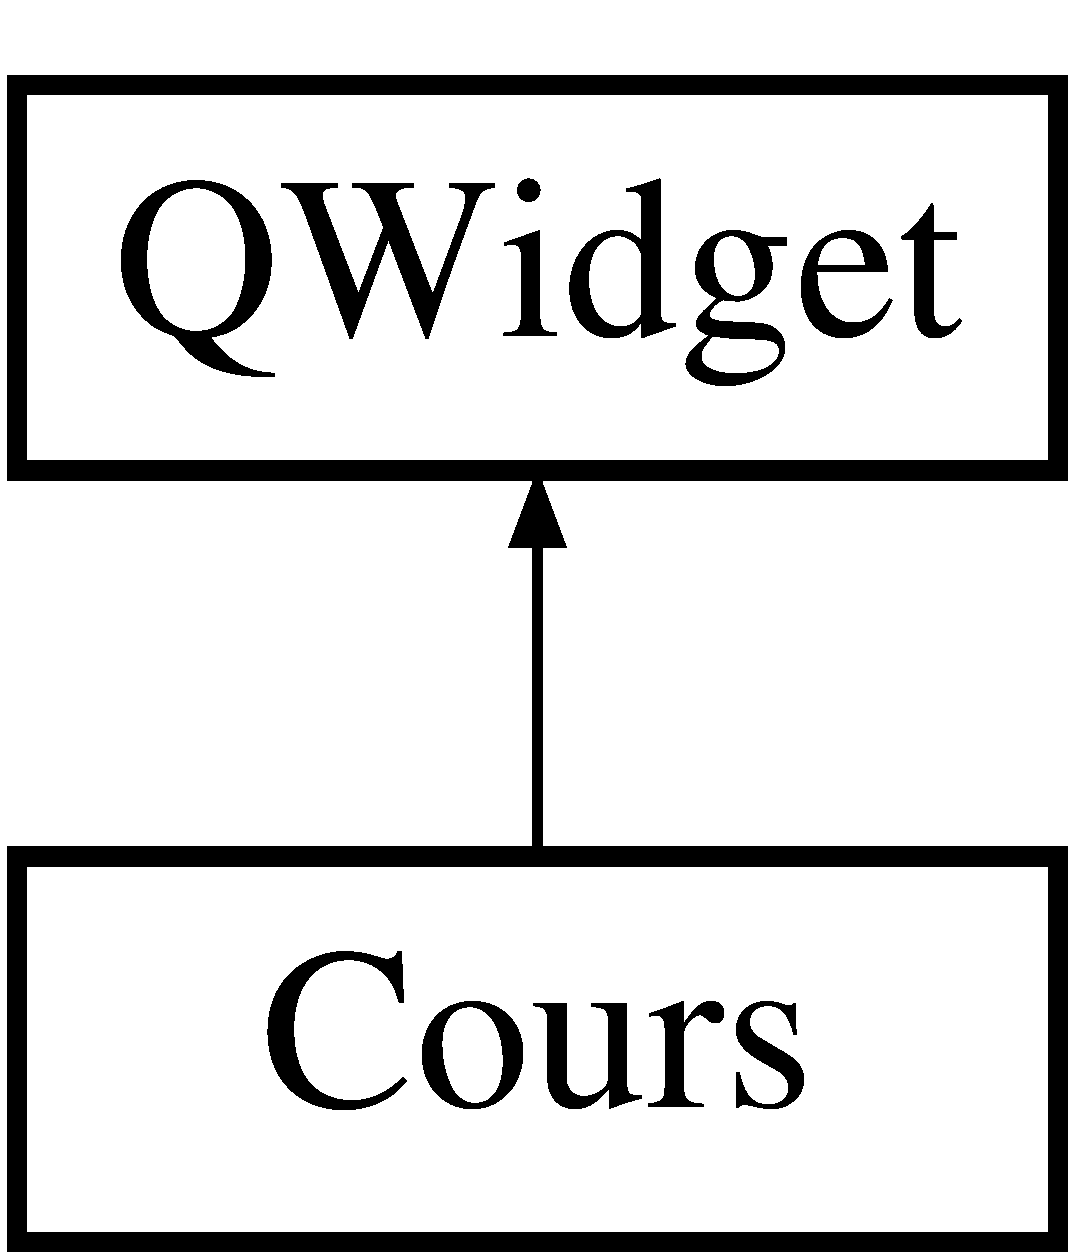
\includegraphics[height=2.000000cm]{class_cours}
\end{center}
\end{figure}
\subsection*{Public Slots}
\begin{DoxyCompactItemize}
\item 
void {\bf go\-Accueil} ()
\begin{DoxyCompactList}\small\item\em Fonction qui permet d'aller sur la fenetre d'accueil. \end{DoxyCompactList}\end{DoxyCompactItemize}
\subsection*{Public Member Functions}
\begin{DoxyCompactItemize}
\item 
{\bf Cours} (Q\-Stacked\-Widget $\ast$pages)
\begin{DoxyCompactList}\small\item\em Constructeur. \end{DoxyCompactList}\end{DoxyCompactItemize}


\subsection{Constructor \& Destructor Documentation}
\index{Cours@{Cours}!Cours@{Cours}}
\index{Cours@{Cours}!Cours@{Cours}}
\subsubsection[{Cours}]{\setlength{\rightskip}{0pt plus 5cm}Cours\-::\-Cours (
\begin{DoxyParamCaption}
\item[{Q\-Stacked\-Widget $\ast$}]{pages}
\end{DoxyParamCaption}
)\hspace{0.3cm}{\ttfamily [explicit]}}\label{class_cours_a36d4fa28603432c36f021d09674b198c}


Constructeur. 


\begin{DoxyParams}{Parameters}
{\em pages} & Pointeur sur la structure de donnée contenant l'ensemble des fenetre, ne peut etre N\-U\-L\-L \\
\hline
\end{DoxyParams}


\subsection{Member Function Documentation}
\index{Cours@{Cours}!go\-Accueil@{go\-Accueil}}
\index{go\-Accueil@{go\-Accueil}!Cours@{Cours}}
\subsubsection[{go\-Accueil}]{\setlength{\rightskip}{0pt plus 5cm}void Cours\-::go\-Accueil (
\begin{DoxyParamCaption}
{}
\end{DoxyParamCaption}
)\hspace{0.3cm}{\ttfamily [slot]}}\label{class_cours_ab6cbed9c1f26daab242a0ea89c696313}


Fonction qui permet d'aller sur la fenetre d'accueil. 


\begin{DoxyParams}{Parameters}
{\em void} & \\
\hline
\end{DoxyParams}


The documentation for this class was generated from the following files\-:\begin{DoxyCompactItemize}
\item 
cours.\-h\item 
cours.\-cpp\end{DoxyCompactItemize}

\section{Entrainement\-Facile Class Reference}
\label{class_entrainement_facile}\index{Entrainement\-Facile@{Entrainement\-Facile}}
Inheritance diagram for Entrainement\-Facile\-:\begin{figure}[H]
\begin{center}
\leavevmode
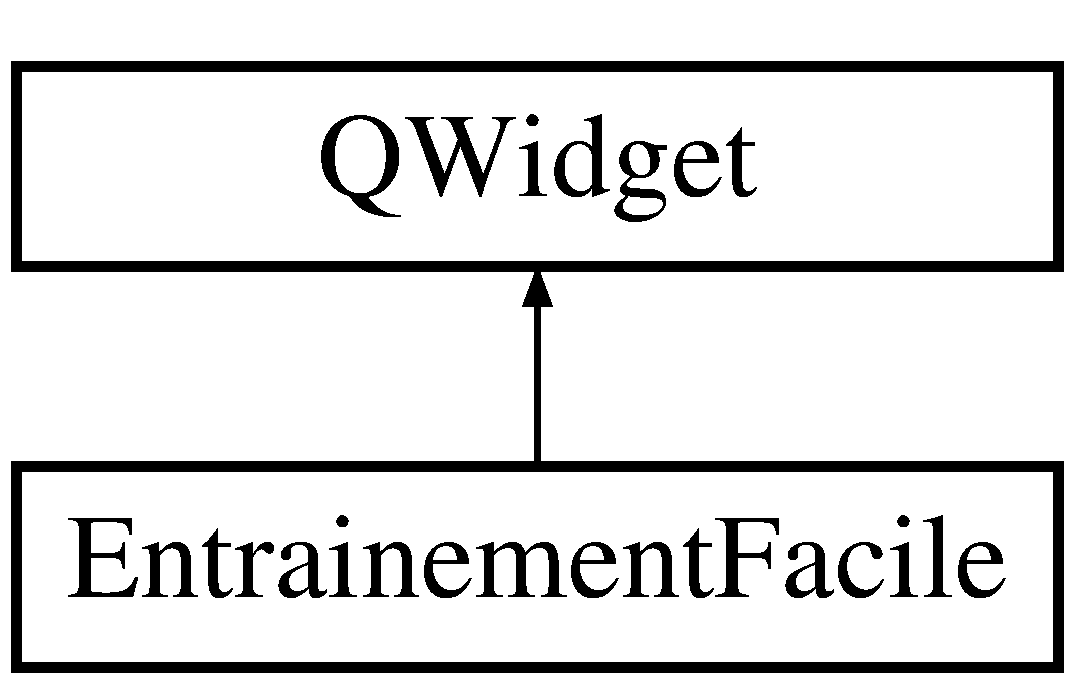
\includegraphics[height=2.000000cm]{class_entrainement_facile}
\end{center}
\end{figure}
\subsection*{Public Slots}
\begin{DoxyCompactItemize}
\item 
void {\bf go\-Accueil} ()
\begin{DoxyCompactList}\small\item\em Fonction qui permet d'aller sur la fenetre d'accueil. \end{DoxyCompactList}\item 
void {\bf appui\-Do1} ()
\begin{DoxyCompactList}\small\item\em Fonction qui déclenche le traitement de la touche do mineur. \end{DoxyCompactList}\item 
void {\bfseries appui\-Do2} ()\label{class_entrainement_facile_afc632a43affef76c28967b624c59a781}

\item 
void {\bf appui\-Re1} ()
\begin{DoxyCompactList}\small\item\em Fonction qui déclenche le traitement de la touche re mineur. \end{DoxyCompactList}\item 
void {\bf appui\-Re2} ()
\begin{DoxyCompactList}\small\item\em Fonction qui déclenche le traitement de la touche re majeur. \end{DoxyCompactList}\item 
void {\bf appui\-Mi1} ()
\begin{DoxyCompactList}\small\item\em Fonction qui déclenche le traitement de la touche mi mineur. \end{DoxyCompactList}\item 
void {\bf appui\-Mi2} ()
\begin{DoxyCompactList}\small\item\em Fonction qui déclenche le traitement de la touche mi majeur. \end{DoxyCompactList}\item 
void {\bf appui\-Fa1} ()
\begin{DoxyCompactList}\small\item\em Fonction qui déclenche le traitement de la touche fa mineur. \end{DoxyCompactList}\item 
void {\bf appui\-Fa2} ()
\begin{DoxyCompactList}\small\item\em Fonction qui déclenche le traitement de la touche fa majeur. \end{DoxyCompactList}\item 
void {\bf appui\-Sol1} ()
\begin{DoxyCompactList}\small\item\em Fonction qui déclenche le traitement de la touche sol mineur. \end{DoxyCompactList}\item 
void {\bf appui\-Sol2} ()
\begin{DoxyCompactList}\small\item\em Fonction qui déclenche le traitement de la touche sol majeur. \end{DoxyCompactList}\item 
void {\bf appui\-La1} ()
\begin{DoxyCompactList}\small\item\em Fonction qui déclenche le traitement de la touche la mineur. \end{DoxyCompactList}\item 
void {\bf appui\-La2} ()
\begin{DoxyCompactList}\small\item\em Fonction qui déclenche le traitement de la touche la majeur. \end{DoxyCompactList}\item 
void {\bf appui\-Si1} ()
\begin{DoxyCompactList}\small\item\em Fonction qui déclenche le traitement de la touche si mineur. \end{DoxyCompactList}\item 
void {\bf appui\-Si2} ()
\begin{DoxyCompactList}\small\item\em Fonction qui déclenche le traitement de la touche si majeur. \end{DoxyCompactList}\item 
void {\bf commencer} ()
\begin{DoxyCompactList}\small\item\em Fonction qui met la partie en place. \end{DoxyCompactList}\item 
void {\bf precedent} ()
\begin{DoxyCompactList}\small\item\em Fonction qui permet de retourner sur la page précédente. \end{DoxyCompactList}\item 
void {\bf compter} ()
\begin{DoxyCompactList}\small\item\em Fonction qui permet le compte à rebours. \end{DoxyCompactList}\end{DoxyCompactItemize}
\subsection*{Public Member Functions}
\begin{DoxyCompactItemize}
\item 
{\bf Entrainement\-Facile} (Q\-Stacked\-Widget $\ast$p)
\begin{DoxyCompactList}\small\item\em Constructeur. \end{DoxyCompactList}\item 
void {\bf paint\-Event} (Q\-Paint\-Event $\ast$e)
\begin{DoxyCompactList}\small\item\em Fonction qui dessine en continue les éléments de l'interface. \end{DoxyCompactList}\item 
void {\bf charger\-Partition} (Q\-String fichier)
\begin{DoxyCompactList}\small\item\em Fonction qui transforme le fichier d'entrée en tableau de notes. \end{DoxyCompactList}\item 
void {\bf placer\-Note} (Q\-Painter \&painter, qreal largeur, qreal hauteur, qreal x\-Debut\-Ligne, qreal y\-Debut\-Ligne, qreal x\-Debut\-Note, qreal espace\-Entre\-Ligne, Q\-String note, Q\-String hauteur\-N)
\begin{DoxyCompactList}\small\item\em Fonction qui dessine une note. \end{DoxyCompactList}\item 
void {\bf deconnection\-Des\-Touches} ()
\begin{DoxyCompactList}\small\item\em Fonction qui déconnecte les touches du clavier afin qu'il n'y ai plus d'action au clique de la souris. \end{DoxyCompactList}\item 
void {\bf partie\-Terminee} ()
\begin{DoxyCompactList}\small\item\em Fonction qui fait la mise à jour de la fenetre lorsque l'entrainement se termine. \end{DoxyCompactList}\item 
void {\bf ecrire\-Log} (Q\-String s)
\begin{DoxyCompactList}\small\item\em Fonction qui ouvre le fichier de log afin d'y ajouter la chaine de caractère passée en paramètre. \end{DoxyCompactList}\item 
void {\bf effacer\-Nom\-Touche} ()
\begin{DoxyCompactList}\small\item\em Fonction qui efface le nom des touches du clavier. \end{DoxyCompactList}\end{DoxyCompactItemize}


\subsection{Constructor \& Destructor Documentation}
\index{Entrainement\-Facile@{Entrainement\-Facile}!Entrainement\-Facile@{Entrainement\-Facile}}
\index{Entrainement\-Facile@{Entrainement\-Facile}!EntrainementFacile@{Entrainement\-Facile}}
\subsubsection[{Entrainement\-Facile}]{\setlength{\rightskip}{0pt plus 5cm}Entrainement\-Facile\-::\-Entrainement\-Facile (
\begin{DoxyParamCaption}
\item[{Q\-Stacked\-Widget $\ast$}]{pages}
\end{DoxyParamCaption}
)\hspace{0.3cm}{\ttfamily [explicit]}}\label{class_entrainement_facile_a7866def70a3208e3676c0f64a9a6f78f}


Constructeur. 


\begin{DoxyParams}{Parameters}
{\em pages} & Pointeur sur la structure de donnée contenant l'ensemble des fenetre, ne peut etre N\-U\-L\-L \\
\hline
\end{DoxyParams}


\subsection{Member Function Documentation}
\index{Entrainement\-Facile@{Entrainement\-Facile}!appui\-Do1@{appui\-Do1}}
\index{appui\-Do1@{appui\-Do1}!EntrainementFacile@{Entrainement\-Facile}}
\subsubsection[{appui\-Do1}]{\setlength{\rightskip}{0pt plus 5cm}void Entrainement\-Facile\-::appui\-Do1 (
\begin{DoxyParamCaption}
{}
\end{DoxyParamCaption}
)\hspace{0.3cm}{\ttfamily [slot]}}\label{class_entrainement_facile_a4f712bbc9e0f50e66f494c916530189d}


Fonction qui déclenche le traitement de la touche do mineur. 


\begin{DoxyParams}{Parameters}
{\em void} & \\
\hline
\end{DoxyParams}
\index{Entrainement\-Facile@{Entrainement\-Facile}!appui\-Fa1@{appui\-Fa1}}
\index{appui\-Fa1@{appui\-Fa1}!EntrainementFacile@{Entrainement\-Facile}}
\subsubsection[{appui\-Fa1}]{\setlength{\rightskip}{0pt plus 5cm}void Entrainement\-Facile\-::appui\-Fa1 (
\begin{DoxyParamCaption}
{}
\end{DoxyParamCaption}
)\hspace{0.3cm}{\ttfamily [slot]}}\label{class_entrainement_facile_a6785c6a1a9491e1ed7c4fb0daad2c54f}


Fonction qui déclenche le traitement de la touche fa mineur. 


\begin{DoxyParams}{Parameters}
{\em void} & \\
\hline
\end{DoxyParams}
\index{Entrainement\-Facile@{Entrainement\-Facile}!appui\-Fa2@{appui\-Fa2}}
\index{appui\-Fa2@{appui\-Fa2}!EntrainementFacile@{Entrainement\-Facile}}
\subsubsection[{appui\-Fa2}]{\setlength{\rightskip}{0pt plus 5cm}void Entrainement\-Facile\-::appui\-Fa2 (
\begin{DoxyParamCaption}
{}
\end{DoxyParamCaption}
)\hspace{0.3cm}{\ttfamily [slot]}}\label{class_entrainement_facile_a51e1165f76cf6cc7b5e092385a3a892c}


Fonction qui déclenche le traitement de la touche fa majeur. 


\begin{DoxyParams}{Parameters}
{\em void} & \\
\hline
\end{DoxyParams}
\index{Entrainement\-Facile@{Entrainement\-Facile}!appui\-La1@{appui\-La1}}
\index{appui\-La1@{appui\-La1}!EntrainementFacile@{Entrainement\-Facile}}
\subsubsection[{appui\-La1}]{\setlength{\rightskip}{0pt plus 5cm}void Entrainement\-Facile\-::appui\-La1 (
\begin{DoxyParamCaption}
{}
\end{DoxyParamCaption}
)\hspace{0.3cm}{\ttfamily [slot]}}\label{class_entrainement_facile_adb0b4da5500d3dd4a691b867ed0d28b0}


Fonction qui déclenche le traitement de la touche la mineur. 


\begin{DoxyParams}{Parameters}
{\em void} & \\
\hline
\end{DoxyParams}
\index{Entrainement\-Facile@{Entrainement\-Facile}!appui\-La2@{appui\-La2}}
\index{appui\-La2@{appui\-La2}!EntrainementFacile@{Entrainement\-Facile}}
\subsubsection[{appui\-La2}]{\setlength{\rightskip}{0pt plus 5cm}void Entrainement\-Facile\-::appui\-La2 (
\begin{DoxyParamCaption}
{}
\end{DoxyParamCaption}
)\hspace{0.3cm}{\ttfamily [slot]}}\label{class_entrainement_facile_a523bae690487d2694829a3c16ff4afab}


Fonction qui déclenche le traitement de la touche la majeur. 


\begin{DoxyParams}{Parameters}
{\em void} & \\
\hline
\end{DoxyParams}
\index{Entrainement\-Facile@{Entrainement\-Facile}!appui\-Mi1@{appui\-Mi1}}
\index{appui\-Mi1@{appui\-Mi1}!EntrainementFacile@{Entrainement\-Facile}}
\subsubsection[{appui\-Mi1}]{\setlength{\rightskip}{0pt plus 5cm}void Entrainement\-Facile\-::appui\-Mi1 (
\begin{DoxyParamCaption}
{}
\end{DoxyParamCaption}
)\hspace{0.3cm}{\ttfamily [slot]}}\label{class_entrainement_facile_a338149b217a871190896940cceb40dfa}


Fonction qui déclenche le traitement de la touche mi mineur. 


\begin{DoxyParams}{Parameters}
{\em void} & \\
\hline
\end{DoxyParams}
\index{Entrainement\-Facile@{Entrainement\-Facile}!appui\-Mi2@{appui\-Mi2}}
\index{appui\-Mi2@{appui\-Mi2}!EntrainementFacile@{Entrainement\-Facile}}
\subsubsection[{appui\-Mi2}]{\setlength{\rightskip}{0pt plus 5cm}void Entrainement\-Facile\-::appui\-Mi2 (
\begin{DoxyParamCaption}
{}
\end{DoxyParamCaption}
)\hspace{0.3cm}{\ttfamily [slot]}}\label{class_entrainement_facile_addd87ab720ba1733862415f426b411dc}


Fonction qui déclenche le traitement de la touche mi majeur. 


\begin{DoxyParams}{Parameters}
{\em void} & \\
\hline
\end{DoxyParams}
\index{Entrainement\-Facile@{Entrainement\-Facile}!appui\-Re1@{appui\-Re1}}
\index{appui\-Re1@{appui\-Re1}!EntrainementFacile@{Entrainement\-Facile}}
\subsubsection[{appui\-Re1}]{\setlength{\rightskip}{0pt plus 5cm}void Entrainement\-Facile\-::appui\-Re1 (
\begin{DoxyParamCaption}
{}
\end{DoxyParamCaption}
)\hspace{0.3cm}{\ttfamily [slot]}}\label{class_entrainement_facile_a46f4bee3e18808bf287510e9b27e06ae}


Fonction qui déclenche le traitement de la touche re mineur. 


\begin{DoxyParams}{Parameters}
{\em void} & \\
\hline
\end{DoxyParams}
\index{Entrainement\-Facile@{Entrainement\-Facile}!appui\-Re2@{appui\-Re2}}
\index{appui\-Re2@{appui\-Re2}!EntrainementFacile@{Entrainement\-Facile}}
\subsubsection[{appui\-Re2}]{\setlength{\rightskip}{0pt plus 5cm}void Entrainement\-Facile\-::appui\-Re2 (
\begin{DoxyParamCaption}
{}
\end{DoxyParamCaption}
)\hspace{0.3cm}{\ttfamily [slot]}}\label{class_entrainement_facile_ac5b5e52a23219ad8924bb86565bffac7}


Fonction qui déclenche le traitement de la touche re majeur. 


\begin{DoxyParams}{Parameters}
{\em void} & \\
\hline
\end{DoxyParams}
\index{Entrainement\-Facile@{Entrainement\-Facile}!appui\-Si1@{appui\-Si1}}
\index{appui\-Si1@{appui\-Si1}!EntrainementFacile@{Entrainement\-Facile}}
\subsubsection[{appui\-Si1}]{\setlength{\rightskip}{0pt plus 5cm}void Entrainement\-Facile\-::appui\-Si1 (
\begin{DoxyParamCaption}
{}
\end{DoxyParamCaption}
)\hspace{0.3cm}{\ttfamily [slot]}}\label{class_entrainement_facile_a08600d1e9b5fc9150ad7958fe4a162b8}


Fonction qui déclenche le traitement de la touche si mineur. 


\begin{DoxyParams}{Parameters}
{\em void} & \\
\hline
\end{DoxyParams}
\index{Entrainement\-Facile@{Entrainement\-Facile}!appui\-Si2@{appui\-Si2}}
\index{appui\-Si2@{appui\-Si2}!EntrainementFacile@{Entrainement\-Facile}}
\subsubsection[{appui\-Si2}]{\setlength{\rightskip}{0pt plus 5cm}void Entrainement\-Facile\-::appui\-Si2 (
\begin{DoxyParamCaption}
{}
\end{DoxyParamCaption}
)\hspace{0.3cm}{\ttfamily [slot]}}\label{class_entrainement_facile_a766e275dbdd993883ed90b282c6d8ebe}


Fonction qui déclenche le traitement de la touche si majeur. 


\begin{DoxyParams}{Parameters}
{\em void} & \\
\hline
\end{DoxyParams}
\index{Entrainement\-Facile@{Entrainement\-Facile}!appui\-Sol1@{appui\-Sol1}}
\index{appui\-Sol1@{appui\-Sol1}!EntrainementFacile@{Entrainement\-Facile}}
\subsubsection[{appui\-Sol1}]{\setlength{\rightskip}{0pt plus 5cm}void Entrainement\-Facile\-::appui\-Sol1 (
\begin{DoxyParamCaption}
{}
\end{DoxyParamCaption}
)\hspace{0.3cm}{\ttfamily [slot]}}\label{class_entrainement_facile_a0300b93cfead2956432d560d614b4788}


Fonction qui déclenche le traitement de la touche sol mineur. 


\begin{DoxyParams}{Parameters}
{\em void} & \\
\hline
\end{DoxyParams}
\index{Entrainement\-Facile@{Entrainement\-Facile}!appui\-Sol2@{appui\-Sol2}}
\index{appui\-Sol2@{appui\-Sol2}!EntrainementFacile@{Entrainement\-Facile}}
\subsubsection[{appui\-Sol2}]{\setlength{\rightskip}{0pt plus 5cm}void Entrainement\-Facile\-::appui\-Sol2 (
\begin{DoxyParamCaption}
{}
\end{DoxyParamCaption}
)\hspace{0.3cm}{\ttfamily [slot]}}\label{class_entrainement_facile_a1456556663003da5f9e42381fd263a8d}


Fonction qui déclenche le traitement de la touche sol majeur. 


\begin{DoxyParams}{Parameters}
{\em void} & \\
\hline
\end{DoxyParams}
\index{Entrainement\-Facile@{Entrainement\-Facile}!charger\-Partition@{charger\-Partition}}
\index{charger\-Partition@{charger\-Partition}!EntrainementFacile@{Entrainement\-Facile}}
\subsubsection[{charger\-Partition}]{\setlength{\rightskip}{0pt plus 5cm}void Entrainement\-Facile\-::charger\-Partition (
\begin{DoxyParamCaption}
\item[{Q\-String}]{fichier}
\end{DoxyParamCaption}
)}\label{class_entrainement_facile_a9cf1e3eb47f58fbb9a1ef5778892217f}


Fonction qui transforme le fichier d'entrée en tableau de notes. 


\begin{DoxyParams}{Parameters}
{\em fichier} & Chemin du fichier xml dans lequel se trouve la partition (doit obligatoirement contenir l'extension .xml) \\
\hline
\end{DoxyParams}
\index{Entrainement\-Facile@{Entrainement\-Facile}!commencer@{commencer}}
\index{commencer@{commencer}!EntrainementFacile@{Entrainement\-Facile}}
\subsubsection[{commencer}]{\setlength{\rightskip}{0pt plus 5cm}void Entrainement\-Facile\-::commencer (
\begin{DoxyParamCaption}
{}
\end{DoxyParamCaption}
)\hspace{0.3cm}{\ttfamily [slot]}}\label{class_entrainement_facile_a3b86785bc5c472f2addd86d6a5f23d58}


Fonction qui met la partie en place. 


\begin{DoxyParams}{Parameters}
{\em void} & \\
\hline
\end{DoxyParams}
\index{Entrainement\-Facile@{Entrainement\-Facile}!compter@{compter}}
\index{compter@{compter}!EntrainementFacile@{Entrainement\-Facile}}
\subsubsection[{compter}]{\setlength{\rightskip}{0pt plus 5cm}void Entrainement\-Facile\-::compter (
\begin{DoxyParamCaption}
{}
\end{DoxyParamCaption}
)\hspace{0.3cm}{\ttfamily [slot]}}\label{class_entrainement_facile_a0d7f12a81700164a4fdb61b70ad64a5c}


Fonction qui permet le compte à rebours. 


\begin{DoxyParams}{Parameters}
{\em void} & \\
\hline
\end{DoxyParams}
\index{Entrainement\-Facile@{Entrainement\-Facile}!deconnection\-Des\-Touches@{deconnection\-Des\-Touches}}
\index{deconnection\-Des\-Touches@{deconnection\-Des\-Touches}!EntrainementFacile@{Entrainement\-Facile}}
\subsubsection[{deconnection\-Des\-Touches}]{\setlength{\rightskip}{0pt plus 5cm}void Entrainement\-Facile\-::deconnection\-Des\-Touches (
\begin{DoxyParamCaption}
{}
\end{DoxyParamCaption}
)}\label{class_entrainement_facile_a04968328b30dba701185f6cb29ebd686}


Fonction qui déconnecte les touches du clavier afin qu'il n'y ai plus d'action au clique de la souris. 

\begin{DoxyReturn}{Returns}
void 
\end{DoxyReturn}
\index{Entrainement\-Facile@{Entrainement\-Facile}!ecrire\-Log@{ecrire\-Log}}
\index{ecrire\-Log@{ecrire\-Log}!EntrainementFacile@{Entrainement\-Facile}}
\subsubsection[{ecrire\-Log}]{\setlength{\rightskip}{0pt plus 5cm}void Entrainement\-Facile\-::ecrire\-Log (
\begin{DoxyParamCaption}
\item[{Q\-String}]{s}
\end{DoxyParamCaption}
)}\label{class_entrainement_facile_a0e38dc4bbe05055ebb9a35e0f7535a4e}


Fonction qui ouvre le fichier de log afin d'y ajouter la chaine de caractère passée en paramètre. 


\begin{DoxyParams}{Parameters}
{\em s} & une chaine de type Q\-String qui sera écrite dans le fichier log, ne peut etre N\-U\-L\-L \\
\hline
\end{DoxyParams}
\begin{DoxyReturn}{Returns}
void 
\end{DoxyReturn}
\index{Entrainement\-Facile@{Entrainement\-Facile}!effacer\-Nom\-Touche@{effacer\-Nom\-Touche}}
\index{effacer\-Nom\-Touche@{effacer\-Nom\-Touche}!EntrainementFacile@{Entrainement\-Facile}}
\subsubsection[{effacer\-Nom\-Touche}]{\setlength{\rightskip}{0pt plus 5cm}Entrainement\-Facile\-::effacer\-Nom\-Touche (
\begin{DoxyParamCaption}
{}
\end{DoxyParamCaption}
)}\label{class_entrainement_facile_a73124bc24183522222fc149ccc36d6e9}


Fonction qui efface le nom des touches du clavier. 

\begin{DoxyReturn}{Returns}
void 
\end{DoxyReturn}
\index{Entrainement\-Facile@{Entrainement\-Facile}!go\-Accueil@{go\-Accueil}}
\index{go\-Accueil@{go\-Accueil}!EntrainementFacile@{Entrainement\-Facile}}
\subsubsection[{go\-Accueil}]{\setlength{\rightskip}{0pt plus 5cm}void Entrainement\-Facile\-::go\-Accueil (
\begin{DoxyParamCaption}
{}
\end{DoxyParamCaption}
)\hspace{0.3cm}{\ttfamily [slot]}}\label{class_entrainement_facile_a84997812d2a67a40a4eab8a05b264438}


Fonction qui permet d'aller sur la fenetre d'accueil. 


\begin{DoxyParams}{Parameters}
{\em void} & \\
\hline
\end{DoxyParams}
\index{Entrainement\-Facile@{Entrainement\-Facile}!paint\-Event@{paint\-Event}}
\index{paint\-Event@{paint\-Event}!EntrainementFacile@{Entrainement\-Facile}}
\subsubsection[{paint\-Event}]{\setlength{\rightskip}{0pt plus 5cm}void Entrainement\-Facile\-::paint\-Event (
\begin{DoxyParamCaption}
\item[{Q\-Paint\-Event $\ast$}]{e}
\end{DoxyParamCaption}
)}\label{class_entrainement_facile_a3b777c927b35947416d98ad7144fe1f8}


Fonction qui dessine en continue les éléments de l'interface. 


\begin{DoxyParams}{Parameters}
{\em e} & Evenement \\
\hline
\end{DoxyParams}
\index{Entrainement\-Facile@{Entrainement\-Facile}!partie\-Terminee@{partie\-Terminee}}
\index{partie\-Terminee@{partie\-Terminee}!EntrainementFacile@{Entrainement\-Facile}}
\subsubsection[{partie\-Terminee}]{\setlength{\rightskip}{0pt plus 5cm}void Entrainement\-Facile\-::partie\-Terminee (
\begin{DoxyParamCaption}
{}
\end{DoxyParamCaption}
)}\label{class_entrainement_facile_a41da1ad2f2d2fc58a9a94f1e95fd7f05}


Fonction qui fait la mise à jour de la fenetre lorsque l'entrainement se termine. 

\begin{DoxyReturn}{Returns}
void 
\end{DoxyReturn}
\index{Entrainement\-Facile@{Entrainement\-Facile}!placer\-Note@{placer\-Note}}
\index{placer\-Note@{placer\-Note}!EntrainementFacile@{Entrainement\-Facile}}
\subsubsection[{placer\-Note}]{\setlength{\rightskip}{0pt plus 5cm}void Entrainement\-Facile\-::placer\-Note (
\begin{DoxyParamCaption}
\item[{Q\-Painter \&}]{painter, }
\item[{qreal}]{largeur, }
\item[{qreal}]{hauteur, }
\item[{qreal}]{x\-Debut\-Ligne, }
\item[{qreal}]{y\-Debut\-Ligne, }
\item[{qreal}]{x\-Debut\-Note, }
\item[{qreal}]{espace\-Entre\-Ligne, }
\item[{Q\-String}]{note, }
\item[{Q\-String}]{hauteur\-N}
\end{DoxyParamCaption}
)}\label{class_entrainement_facile_aa9bf53aa869146a1f4375eee0fc219a2}


Fonction qui dessine une note. 


\begin{DoxyParams}{Parameters}
{\em \&painter} & le Q\-Painter sur lequel sera dessiné la note \\
\hline
{\em largeur} & largeur de la fenetre \\
\hline
{\em hauteur} & hauteur de la fenetre \\
\hline
{\em x\-Debut\-Ligne} & Coordonnée x de la premiere ligne de la portee \\
\hline
{\em y\-Debut\-Ligne} & Coordonnée y de la premiere ligne de la portee \\
\hline
{\em x\-Debut\-Note} & Coordonnée x de la ou va etre dessiné la note \\
\hline
{\em espace\-Entre\-Ligne} & Distance entre deux lignes de la portee \\
\hline
{\em note} & Nom de la note à dessiner \\
\hline
{\em hauteur\-N} & Hauteur de la note à dessiner\\
\hline
\end{DoxyParams}
\begin{DoxyReturn}{Returns}
void 
\end{DoxyReturn}
\index{Entrainement\-Facile@{Entrainement\-Facile}!precedent@{precedent}}
\index{precedent@{precedent}!EntrainementFacile@{Entrainement\-Facile}}
\subsubsection[{precedent}]{\setlength{\rightskip}{0pt plus 5cm}void Entrainement\-Facile\-::precedent (
\begin{DoxyParamCaption}
{}
\end{DoxyParamCaption}
)\hspace{0.3cm}{\ttfamily [slot]}}\label{class_entrainement_facile_ae88750334f9bdb0d1736efa16116d2c3}


Fonction qui permet de retourner sur la page précédente. 


\begin{DoxyParams}{Parameters}
{\em void} & \\
\hline
\end{DoxyParams}


The documentation for this class was generated from the following files\-:\begin{DoxyCompactItemize}
\item 
entrainementfacile.\-h\item 
entrainementfacile.\-cpp\end{DoxyCompactItemize}

\section{Référence de la classe Entrainement\-Page1}
\label{class_entrainement_page1}\index{Entrainement\-Page1@{Entrainement\-Page1}}
Graphe d'héritage de Entrainement\-Page1\-:\begin{figure}[H]
\begin{center}
\leavevmode
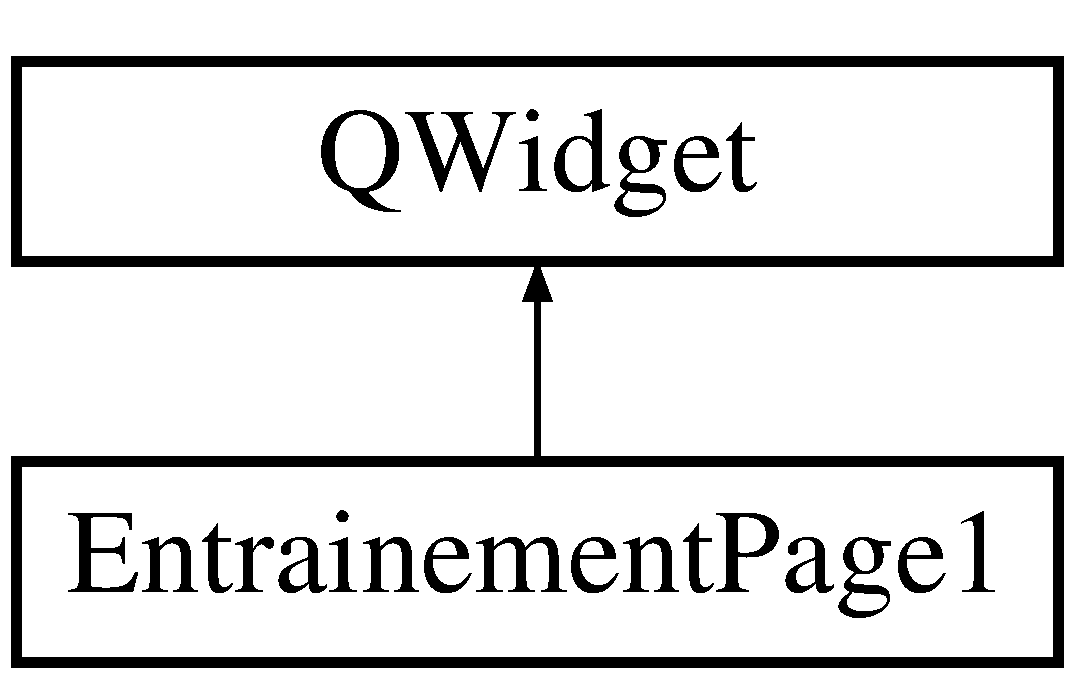
\includegraphics[height=2.000000cm]{class_entrainement_page1}
\end{center}
\end{figure}
\subsection*{Connecteurs publics}
\begin{DoxyCompactItemize}
\item 
void {\bf do\-Facile} ()\label{class_entrainement_page1_aee45c5abd549739198a42206db0eb869}

\begin{DoxyCompactList}\small\item\em Fonction qui permet d'aller à la fenetre d'entrainement en mode facile. \end{DoxyCompactList}\item 
void {\bf do\-Difficile} ()\label{class_entrainement_page1_a6d9fb6299b60a36569fe21202995fa20}

\begin{DoxyCompactList}\small\item\em Fonction qui permet d'aller à la fenetre d'entrainement en mode difficile. \end{DoxyCompactList}\item 
void {\bf go\-Accueil} ()\label{class_entrainement_page1_a27861dfdf502f6edae27f650cba4399c}

\begin{DoxyCompactList}\small\item\em Fonction qui permet de retourner à l'accueil. \end{DoxyCompactList}\item 
void {\bf choix\-Partition} ()\label{class_entrainement_page1_a5350caf23183fcd9e52b5ab06c738454}

\begin{DoxyCompactList}\small\item\em fonction qui permet l'entrainement possible après sélection de la partition \end{DoxyCompactList}\item 
void {\bf insert\-Fichier} (Q\-String s)
\begin{DoxyCompactList}\small\item\em Permet d'ajouter dans un fichier une chaine de caractère. \end{DoxyCompactList}\item 
void {\bf ecrire\-Log} (Q\-String s)
\begin{DoxyCompactList}\small\item\em Fonction qui ouvre le fichier de log afin d'y ajouter la chaine de caractère passée en paramètre. \end{DoxyCompactList}\end{DoxyCompactItemize}
\subsection*{Fonctions membres publiques}
\begin{DoxyCompactItemize}
\item 
{\bf Entrainement\-Page1} (Q\-Stacked\-Widget $\ast$p)
\begin{DoxyCompactList}\small\item\em Constructeur. \end{DoxyCompactList}\item 
void {\bf paint\-Event} (Q\-Paint\-Event $\ast$e)
\begin{DoxyCompactList}\small\item\em Fonction qui dessine les éléments graphiques. \end{DoxyCompactList}\end{DoxyCompactItemize}


\subsection{Documentation des constructeurs et destructeur}
\index{Entrainement\-Page1@{Entrainement\-Page1}!Entrainement\-Page1@{Entrainement\-Page1}}
\index{Entrainement\-Page1@{Entrainement\-Page1}!EntrainementPage1@{Entrainement\-Page1}}
\subsubsection[{Entrainement\-Page1}]{\setlength{\rightskip}{0pt plus 5cm}Entrainement\-Page1\-::\-Entrainement\-Page1 (
\begin{DoxyParamCaption}
\item[{Q\-Stacked\-Widget $\ast$}]{p}
\end{DoxyParamCaption}
)\hspace{0.3cm}{\ttfamily [explicit]}}\label{class_entrainement_page1_ae5daa72fc7c7594f3df82562fe415918}


Constructeur. 


\begin{DoxyParams}{Paramètres}
{\em p} & \\
\hline
\end{DoxyParams}


\subsection{Documentation des fonctions membres}
\index{Entrainement\-Page1@{Entrainement\-Page1}!ecrire\-Log@{ecrire\-Log}}
\index{ecrire\-Log@{ecrire\-Log}!EntrainementPage1@{Entrainement\-Page1}}
\subsubsection[{ecrire\-Log}]{\setlength{\rightskip}{0pt plus 5cm}void Entrainement\-Page1\-::ecrire\-Log (
\begin{DoxyParamCaption}
\item[{Q\-String}]{s}
\end{DoxyParamCaption}
)\hspace{0.3cm}{\ttfamily [slot]}}\label{class_entrainement_page1_a057bff42d565a935fe62a1fb47d891e2}


Fonction qui ouvre le fichier de log afin d'y ajouter la chaine de caractère passée en paramètre. 


\begin{DoxyParams}{Paramètres}
{\em s} & une chaine de type Q\-String qui sera écrite dans le fichier log, ne peut etre N\-U\-L\-L \\
\hline
\end{DoxyParams}
\begin{DoxyReturn}{Renvoie}
void 
\end{DoxyReturn}
\index{Entrainement\-Page1@{Entrainement\-Page1}!insert\-Fichier@{insert\-Fichier}}
\index{insert\-Fichier@{insert\-Fichier}!EntrainementPage1@{Entrainement\-Page1}}
\subsubsection[{insert\-Fichier}]{\setlength{\rightskip}{0pt plus 5cm}void Entrainement\-Page1\-::insert\-Fichier (
\begin{DoxyParamCaption}
\item[{Q\-String}]{s}
\end{DoxyParamCaption}
)\hspace{0.3cm}{\ttfamily [slot]}}\label{class_entrainement_page1_a16afa3244ff5d3fe0bfebcdf81e6c054}


Permet d'ajouter dans un fichier une chaine de caractère. 


\begin{DoxyParams}{Paramètres}
{\em chaine} & de caractère à insérer \\
\hline
\end{DoxyParams}
\index{Entrainement\-Page1@{Entrainement\-Page1}!paint\-Event@{paint\-Event}}
\index{paint\-Event@{paint\-Event}!EntrainementPage1@{Entrainement\-Page1}}
\subsubsection[{paint\-Event}]{\setlength{\rightskip}{0pt plus 5cm}void Entrainement\-Page1\-::paint\-Event (
\begin{DoxyParamCaption}
\item[{Q\-Paint\-Event $\ast$}]{e}
\end{DoxyParamCaption}
)}\label{class_entrainement_page1_ad7099fd9412b8f91aecf47bed03c7935}


Fonction qui dessine les éléments graphiques. 


\begin{DoxyParams}{Paramètres}
{\em e} & un évènement \\
\hline
\end{DoxyParams}


La documentation de cette classe a été générée à partir des fichiers suivants \-:\begin{DoxyCompactItemize}
\item 
entrainementpage1.\-h\item 
entrainementpage1.\-cpp\end{DoxyCompactItemize}

\section{Référence de la classe Fenetre}
\label{class_fenetre}\index{Fenetre@{Fenetre}}
Graphe d'héritage de Fenetre\-:\begin{figure}[H]
\begin{center}
\leavevmode
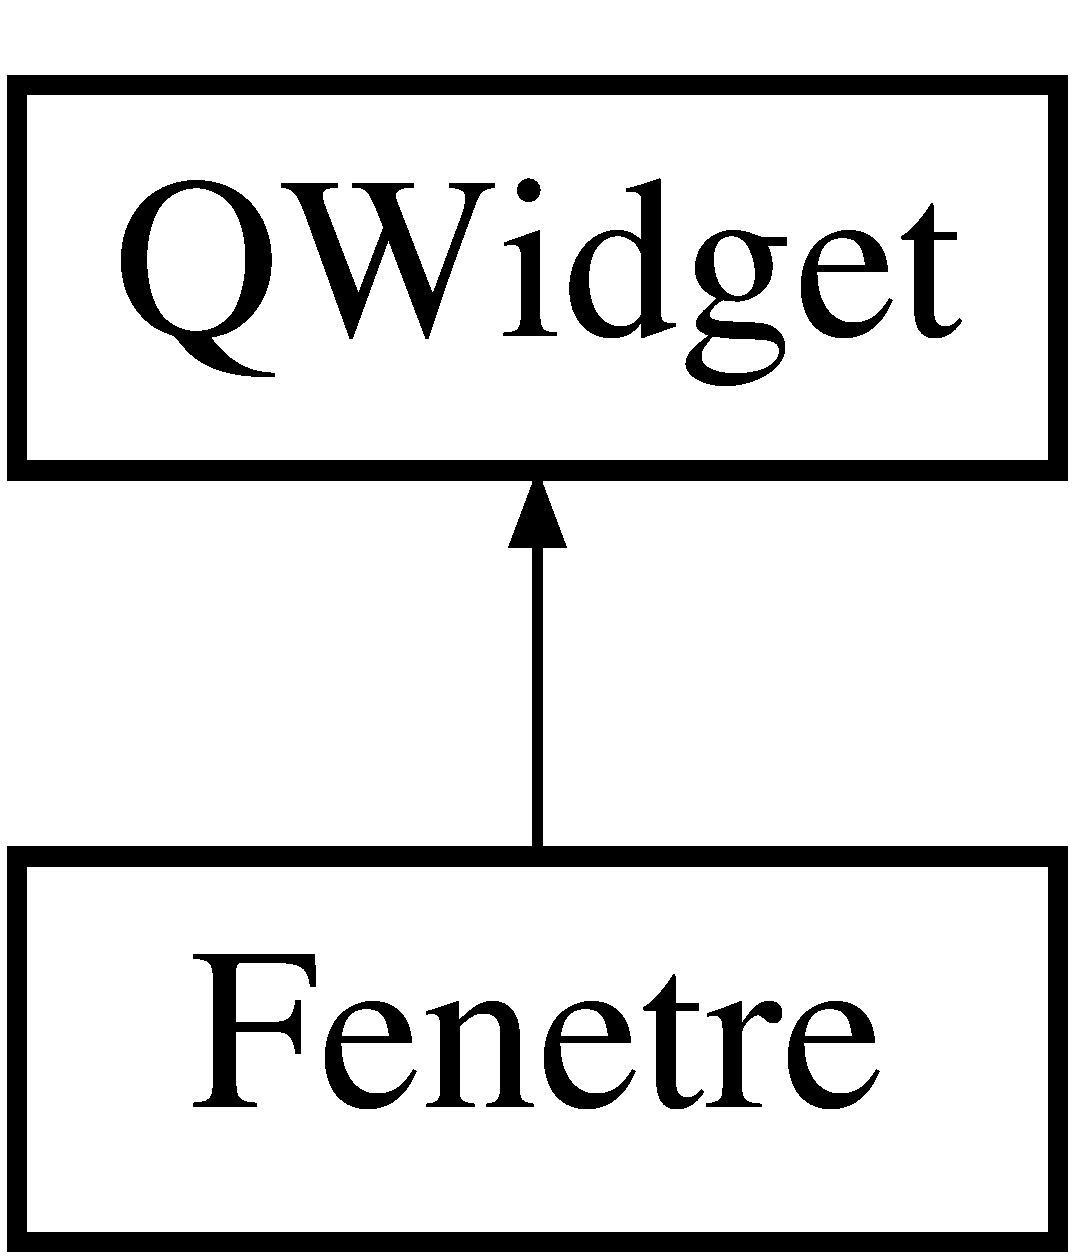
\includegraphics[height=2.000000cm]{class_fenetre}
\end{center}
\end{figure}
\subsection*{Fonctions membres publiques}
\begin{DoxyCompactItemize}
\item 
{\bf Fenetre} (Q\-Widget $\ast$parent=0)
\begin{DoxyCompactList}\small\item\em Constructeur. \end{DoxyCompactList}\end{DoxyCompactItemize}


\subsection{Documentation des constructeurs et destructeur}
\index{Fenetre@{Fenetre}!Fenetre@{Fenetre}}
\index{Fenetre@{Fenetre}!Fenetre@{Fenetre}}
\subsubsection[{Fenetre}]{\setlength{\rightskip}{0pt plus 5cm}Fenetre\-::\-Fenetre (
\begin{DoxyParamCaption}
\item[{Q\-Widget $\ast$}]{parent = {\ttfamily 0}}
\end{DoxyParamCaption}
)\hspace{0.3cm}{\ttfamily [explicit]}}\label{class_fenetre_a783cbd996724ab575651bfb7efd08d8a}


Constructeur. 


\begin{DoxyParams}{Paramètres}
{\em parent} & \\
\hline
\end{DoxyParams}


La documentation de cette classe a été générée à partir des fichiers suivants \-:\begin{DoxyCompactItemize}
\item 
fenetre.\-h\item 
fenetre.\-cpp\end{DoxyCompactItemize}

\section{Jeu\-Libre Class Reference}
\label{class_jeu_libre}\index{Jeu\-Libre@{Jeu\-Libre}}
Inheritance diagram for Jeu\-Libre\-:\begin{figure}[H]
\begin{center}
\leavevmode
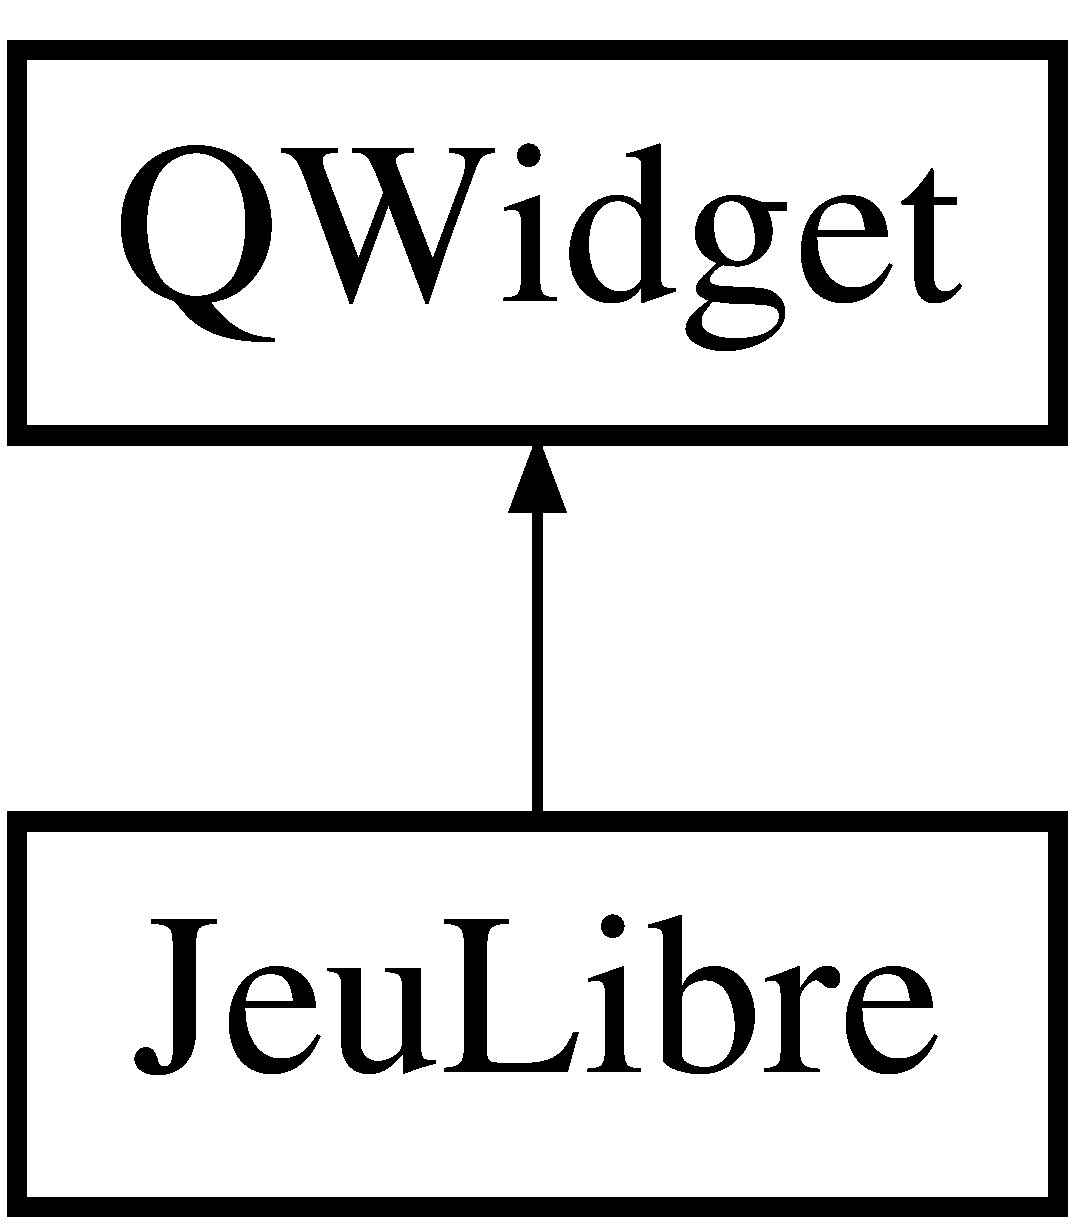
\includegraphics[height=2.000000cm]{class_jeu_libre}
\end{center}
\end{figure}
\subsection*{Public Slots}
\begin{DoxyCompactItemize}
\item 
void {\bfseries go\-Accueil} ()\label{class_jeu_libre_a1d1f4bb8aef07077f7c94c3859d92bc1}

\end{DoxyCompactItemize}
\subsection*{Public Member Functions}
\begin{DoxyCompactItemize}
\item 
{\bf Jeu\-Libre} (Q\-Stacked\-Widget $\ast$p)
\begin{DoxyCompactList}\small\item\em Constructeur. \end{DoxyCompactList}\end{DoxyCompactItemize}


\subsection{Constructor \& Destructor Documentation}
\index{Jeu\-Libre@{Jeu\-Libre}!Jeu\-Libre@{Jeu\-Libre}}
\index{Jeu\-Libre@{Jeu\-Libre}!JeuLibre@{Jeu\-Libre}}
\subsubsection[{Jeu\-Libre}]{\setlength{\rightskip}{0pt plus 5cm}Jeu\-Libre\-::\-Jeu\-Libre (
\begin{DoxyParamCaption}
\item[{Q\-Stacked\-Widget $\ast$}]{p}
\end{DoxyParamCaption}
)\hspace{0.3cm}{\ttfamily [explicit]}}\label{class_jeu_libre_ad325cede424f742aa6d865c5dd638d5a}


Constructeur. 


\begin{DoxyParams}{Parameters}
{\em p} & la structeur contenant les différentes fenetres \\
\hline
\end{DoxyParams}


The documentation for this class was generated from the following files\-:\begin{DoxyCompactItemize}
\item 
jeulibre.\-h\item 
jeulibre.\-cpp\end{DoxyCompactItemize}

\section{Note Class Reference}
\label{class_note}\index{Note@{Note}}
\subsection*{Public Member Functions}
\begin{DoxyCompactItemize}
\item 
{\bf Note} (Q\-String {\bf nom}, Q\-String {\bf hauteur})
\begin{DoxyCompactList}\small\item\em Constructeur. \end{DoxyCompactList}\end{DoxyCompactItemize}
\subsection*{Public Attributes}
\begin{DoxyCompactItemize}
\item 
Q\-String {\bf nom}\label{class_note_a5b91b148f84290ba298e82b4cf1bce92}

\begin{DoxyCompactList}\small\item\em Chaine de caractère contenant le nom de la note. \end{DoxyCompactList}\item 
Q\-String {\bf hauteur}\label{class_note_a0d0fc6ec642de04f3b8d6ce32b7f1bcb}

\begin{DoxyCompactList}\small\item\em Chaine de caractère contenant la hauteur de la note. \end{DoxyCompactList}\end{DoxyCompactItemize}


\subsection{Constructor \& Destructor Documentation}
\index{Note@{Note}!Note@{Note}}
\index{Note@{Note}!Note@{Note}}
\subsubsection[{Note}]{\setlength{\rightskip}{0pt plus 5cm}Note\-::\-Note (
\begin{DoxyParamCaption}
\item[{Q\-String}]{nom, }
\item[{Q\-String}]{hauteur}
\end{DoxyParamCaption}
)}\label{class_note_ac276bbe211c603a7ce8fc701761d03ea}


Constructeur. 


\begin{DoxyParams}{Parameters}
{\em nom} & Nom de la note, ne peut etre N\-U\-L\-L \\
\hline
{\em hauteur} & Hauteur de la note (mineur ou majeur), ne peut etre N\-U\-L\-L \\
\hline
\end{DoxyParams}


The documentation for this class was generated from the following files\-:\begin{DoxyCompactItemize}
\item 
note.\-h\item 
note.\-cpp\end{DoxyCompactItemize}

%--- End generated contents ---

% Index
\newpage
\phantomsection
\addcontentsline{toc}{chapter}{Index}
\printindex

\end{document}
